\section{STARIMA}
\subsection{Stasioner Data}
\label{bab:stasioner-data-starima}
Setelah dilakukan analisis dekomposisi untuk mengidentifikasi pola tren dan musiman, langkah selanjutnya adalah menguji tingkat kestasioneran data pada masing - masing wilayah.
Uji stasioneritas dilakukan untuk memastikan bahwa deret waktu curah hujan telah memenuhi asumsi dasar analisis time series, yaitu nilai rata - rata dan varians yang relatif konstan terhadap waktu.
Data yang tidak stasioner dapat menyebabkan estimasi parameter model menjadi bias dan tidak stabil, sehingga perlu dilakukan transformasi atau differencing sebelum proses pemodelan.
Oleh karena itu, pada tahap ini dilakukan pengujian kestasioneran data curah hujan di kelima wilayah Kota Surabaya guna menentukan apakah proses differencing diperlukan untuk menjadikan data stasioner secara statistik.
\begin{enumerate}[label=\Alph*.]
    \item Kestasioneran terhadap varians \\
    Kestasioneran data curah hujan terhadap varians dapat dilihat dari transformasi lambda $(\lambda)$ yang dihasilkan dari plot BoxCox.
    Jika nilai $(\lambda)$ mendekati satu maka dapat disimpulkan bahwa data telah stasioner dan sebaliknya. Untuk membuat plot BoxCox data yang digunakan harus bernilai positif.
    \begin{table}[H]
    \centering
    \caption{Nilai Lambda Semua Wilayah}
    \label{table:nilai-lambda-semua-wilayah-starima}
    \begin{tabular}{l c}
        \toprule
        \textbf{Wilayah} & \textbf{Nilai Lambda} \\
        \midrule
        Barat   & 0.1962 \\
        Selatan & 0.2009 \\
        Tengah  & 0.1847 \\
        Timur   & 0.1843 \\
        Utara   & 0.1894 \\
        \bottomrule
    \end{tabular}
\end{table}
    Berdasarkan Tabel~\ref{table:nilai-lambda-semua-wilayah-starima} itu nilai $\lambda$ hasil transformasi BoxCox menunjukkan peningkatan yang signifikan pada seluruh wilayah setelah proses optimasi dilakukan.
    Kenaikan nilai $\lambda$ yang mendekati 1 menandakan bahwa varians data curah hujan menjadi lebih stabil dan mendekati kondisi stasioner.
    Dengan demikian, transformasi BoxCox terbukti efektif sebagai langkah pra pemrosesan untuk menormalkan varians dan memastikan bahwa data memenuhi asumsi homoskedastisitas sebelum proses differencing dan pemodelan STARIMA dilakukan.

    \item Kestasioneran terhadap rata - rata \\
    Setelah data stasioner terhadap varians, selanjutnya dilakukan pengujian kestasioneran terhadap rata - rata.
    Pengujian ini dapat dilakukan dengan Menggunakan \textit{Augmented Dickey-Fuller Unit Root Test}, berikut adalah hipotesisnya:
    $H_0:\ \phi \ge 0$ (data tidak stasioner terhadap rata-rata) \text{ vs } 
    $H_1:\ \phi < 0$ (data stasioner terhadap rata-rata)
    Hasil pengujian \textit{Augmented Dickey-Fuller Unit Root} untuk masing-masing lokasi terangkum pada tabel dibawah ini:
    \begin{table}[H]
    \centering
    \caption{Hasil Uji ADF}
    \label{table:hasil-uji-adf-starima}
    \renewcommand{\arraystretch}{1.2}
    \begin{tabular}{lcc}
        \toprule
        \textbf{Wilayah} & \textit{t-statistik} & \textbf{Nilai-p} \\
        \midrule
        Barat   & -8.314 & 0.01 \\
        Selatan & -8.111 & 0.01 \\
        Tengah  & -8.107 & 0.01 \\
        Timur   & -7.781 & 0.01 \\
        Utara   & -8.313 & 0.01 \\
        \bottomrule
    \end{tabular}
\end{table}
    Tabel~\ref{table:hasil-uji-adf-starima} menunjukkan bahwa data curah hujan kelima wilayah Surabaya telah stasioner terhadap varians juga stasioner terhadap rata - rata sehingga tidak perlu di diferensiasi.
    Hal tersebut dapat diketahui dari nilai peluang yang dihasilkan oleh ke 5 wilayah Surabaya yaitu sebesar 0.01.
    Dengan tingkat kepercayaan 95\% dapat disimpulkan bahwa kelima wilayah Surabaya telah stasioner terhadap varians juga stasioner terhadap rata-rata.

    Berikut adalah grafik curah hujan kelima wilayah surabaya setelah dilakukan transformasi BoxCox dan differencing.
    \begin{figure}[H]
        \centering
        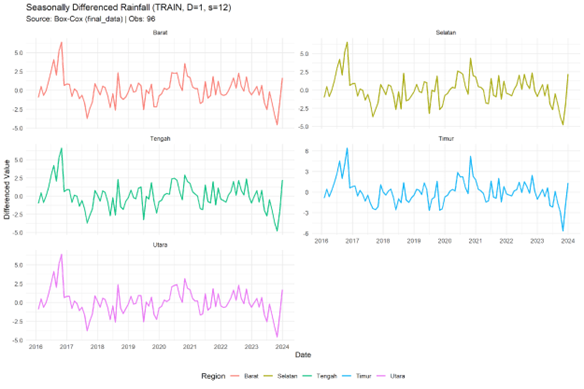
\includegraphics[width=0.9\textwidth]{images/bab_4/bab_4.3/hasil-curah-hujan-setelah-transformasi-dan-differencing.png}
        \caption{Hasil Grafik Curah Hujan Setelah Transformasi dan Differencing}
        \label{fig:hasil-grafik-curah-hujan-starima}
    \end{figure}
    Berdasarkan Gambar~\ref{fig:hasil-grafik-curah-hujan-starima} diatas pola curah hujan yang telah melalui proses differencing musiman, setelah transformasi BoxCox diterapkan.
    Seluruh wilayah Barat, Selatan, Tengah, Timur, dan Utara menunjukkan fluktuasi yang lebih stabil serta tidak lagi memperlihatkan pola musiman yang berulang, menandakan bahwa komponen musiman berhasil dieliminasi.
    Pola residual yang berosilasi di sekitar nol mengindikasikan bahwa data telah berada dalam kondisi yang lebih mendekati stasioner, sehingga layak digunakan untuk pemodelan STARIMA pada tahap selanjutnya.
\end{enumerate}
\subsection{Bobot Seragam}
Pada STARIMA ini setelah melakukan stasioner tes seperti pada poin~\ref{bab:stasioner-data-starima} lalu membuat pembobotan yang mana disini menggunakan tiga pembobotan yaitu bobot lokasi seragam, bobot lokasi invers jarak, dan bobot lokasi normalisasi korelasi silang.
Penggunaan ketiga bobot ini dilakukan untuk mendapatkan model STARIMA terbaik dengan bobot lokasi yang sesuai. 
Berikut merupakan matriks bobot lokasi seragam:
\begin{equation}
    \label{swm-bobot-seragam}
    W = 
    \begin{pmatrix}
        0.00 & 0.25 & 0.25 & 0.25 & 0.25 \\
        0.25 & 0.00 & 0.25 & 0.25 & 0.25 \\
        0.25 & 0.25 & 0.00 & 0.25 & 0.25 \\
        0.25 & 0.25 & 0.25 & 0.00 & 0.25 \\
        0.25 & 0.25 & 0.25 & 0.25 & 0.00 \\
    \end{pmatrix}
\end{equation}
\begin{enumerate}[label=\Alph*.]
    \item Identifikasi \\
    Setelah mendapatkan bobot, melakukan perhitungan STACF seperti pada Rumus~\ref{st_ma} dan STPACF seperti pada Rumus~\ref{st_ar}.
    Perhitungan STACF dan STPACF ini digunakan untuk menentukan orde $p$, $q$ nya karena data nya sudah di differencing.
    Berikut adalah plot STACF dan STPACF:
    \begin{figure}[H]
        \centering
        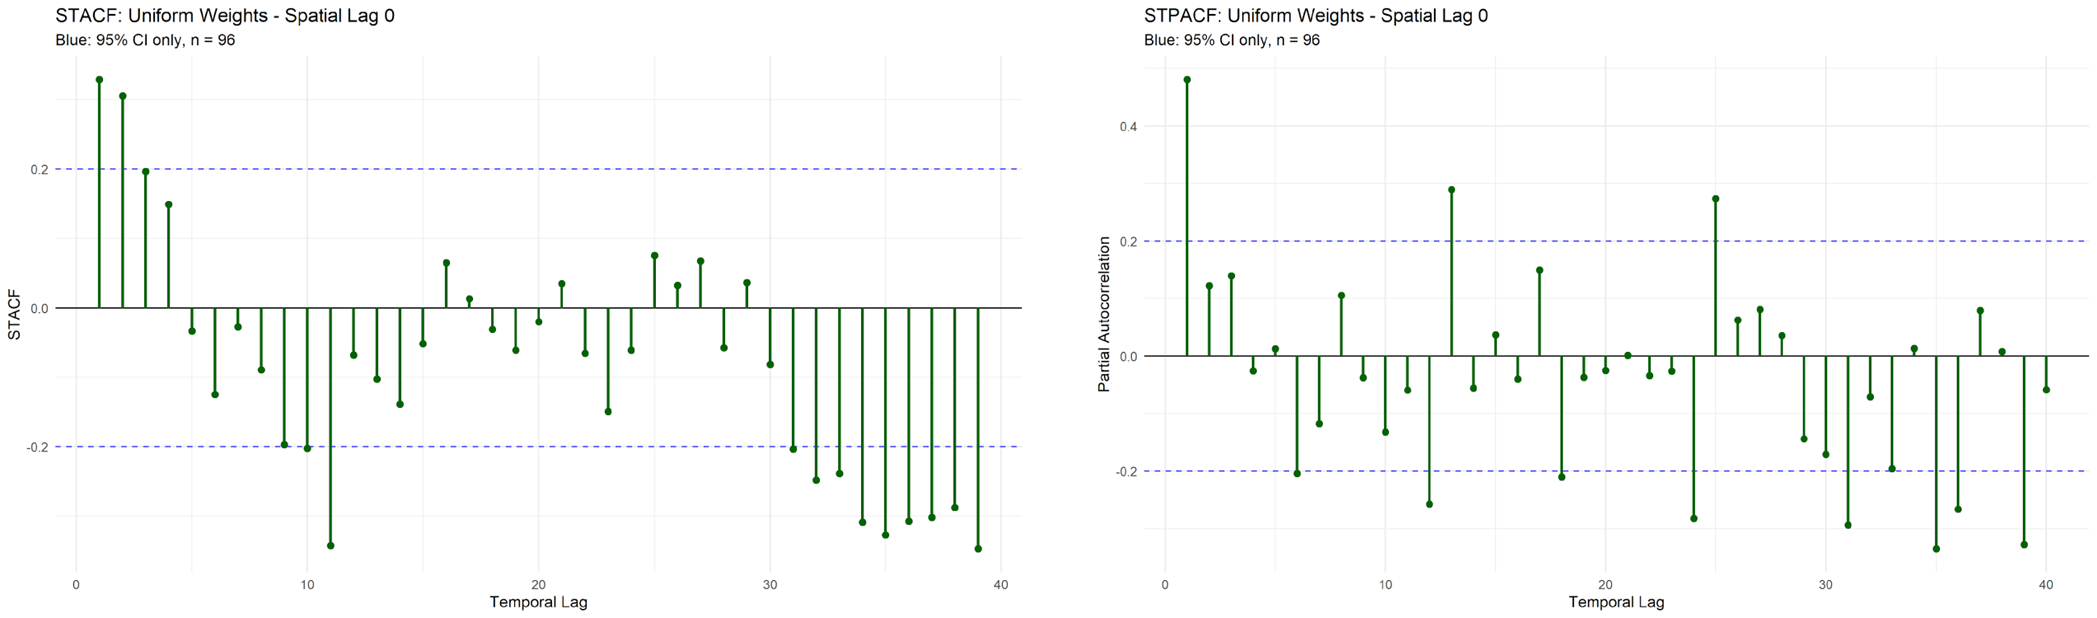
\includegraphics[width=0.9\textwidth]{images/bab_4/bab_4.3/bab_4.3.2/slag-0.png}
        \caption{STACF dan STPACF SLAG 0}
        \label{fig:slag-0-uniform}
    \end{figure}
    Gambar~\ref{fig:slag-0-uniform} menunjukkan hasil analisis \textit{Spatio-Temporal Autocorrelation Function} (STACF) dan \textit{Spatio Temporal Partial Autocorrelation Function} (STPACF) menggunakan bobot seragam.
    Plot STACF pada spatial lag 0 menunjukkan adanya autokorelasi signifikan pada beberapa lag awal yang meluruh secara bertahap tanpa cut-off yang jelas, mengindikasikan dominasi komponen autoregressive.
    Sementara itu, STPACF memperlihatkan spike signifikan yang kuat pada lag 1 dan tidak signifikan pada lag berikutnya, yang merupakan ciri khas proses AR orde rendah.
    Berdasarkan pola tersebut, model dengan komponen AR(1) tanpa komponen MA yang dominan dinilai paling sesuai untuk merepresentasikan struktur temporal data pada spatial lag 0 dengan pembobotan seragam.
    \begin{figure}[H]
        \centering
        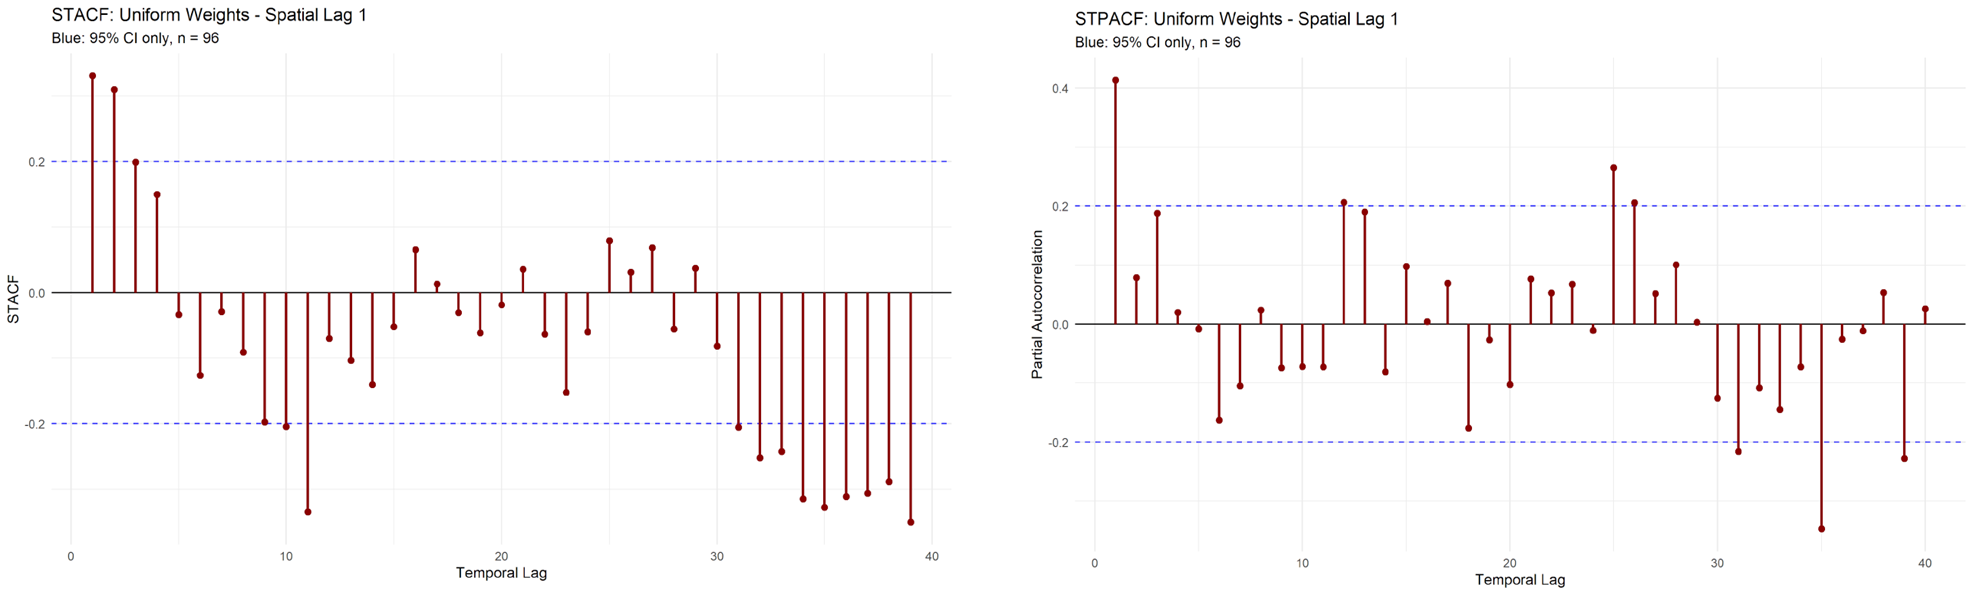
\includegraphics[width=0.9\textwidth]{images/bab_4/bab_4.3/bab_4.3.2/slag-1.png}
        \caption{STACF dan STPACF SLAG 1}
        \label{fig:slag-1-uniform}
    \end{figure}
    Gambar~\ref{fig:slag-1-uniform} menunjukkan hasil analisis \textit{Spatio-Temporal Autocorrelation Function} (STACF) dan \textit{Spatio Temporal Partial Autocorrelation Function} (STPACF) menggunakan bobot seragam.
    Plot STACF pada spatial lag 1 dengan pembobotan seragam menunjukkan adanya autokorelasi signifikan pada beberapa lag awal yang meluruh secara bertahap, mengindikasikan keberadaan ketergantungan spasio-temporal yang kuat.
    Hal ini menandakan bahwa nilai pengamatan pada suatu wilayah dipengaruhi oleh nilai rata-rata wilayah tetangga pada waktu sebelumnya.
    Sementara itu, STPACF memperlihatkan spike signifikan yang dominan pada lag 1 dan tidak signifikan pada lag berikutnya, yang merupakan ciri proses autoregressive orde satu.
    Berdasarkan pola tersebut, model STARIMA dengan komponen AR spasial orde satu dan tanpa komponen MA yang dominan dinilai paling sesuai untuk merepresentasikan struktur spasio-temporal data.
    
    \item Estimasi Parameter \\
    Parameter yang diestimasi dari model yang telah diidentifikasi yaitu STARIMA $(0,0,1) \times (1,1,1)_{12}$ dan STARIMA $(0,0,0) \times (0,1,1_{0})_{12}$ menggunakan metode Maximum Likelihood, disajikan dalam Tabel~\ref{table:estimasi-paramater-starima-uniform}, bersama dengan standar error, nilai $t$, dan nilai $p$ masing-masing:
    \begin{table}[H]
    \centering
    \scriptsize
    \caption{Estimasi Parameter}
    \label{table:estimasi-paramater-starima-uniform}
    \renewcommand{\arraystretch}{1.25}

    \resizebox{\textwidth}{!}{
        \begin{tabular}{|c|c|c|ccc|ccc|}
            \hline
            \multirow{2}{*}{\textbf{Spatial Orde}} &
            \multirow{2}{*}{\textbf{Model}} &
            \multirow{2}{*}{\textbf{Statistik}} &
            \multicolumn{3}{c|}{\textbf{AR Parameter}} &
            \multicolumn{3}{c|}{\textbf{MA Parameter}} \\
            \cline{4-9}

            & & &
            \multicolumn{1}{c|}{$\phi_{10}$} &
            \multicolumn{1}{c|}{$\Phi_{20}$} &
            \multicolumn{1}{c|}{$\Phi_{30}$} &
            \multicolumn{1}{c|}{$\Theta_{10}$} &
            \multicolumn{1}{c|}{$\Theta_{20}$} &
            $\Theta_{30}$ \\
            \hline

            % ================= LAG 0 ========================
            \multirow{12}{*}{Lag 0}
            & \multirow{4}{*}{1,1,0}
            & Estimasi & 0.4812 &  &  &  &  &  \\ \cline{3-9}
            & & SE       & 0.0435 &  &  &  &  &  \\ \cline{3-9}
            & & t-value  & 11.1   &  &  &  &  &  \\ \cline{3-9}
            & & p-value  & $<0.000000000000002$ *** & & & & & \\ \cline{2-9}

            & \multirow{4}{*}{1,1,1}
            & Estimasi & 0.5747 &  &  & -0.1557 &  &  \\ \cline{3-9}
            & & SE       & 0.0685 &  &  & 0.0853 &  &  \\ \cline{3-9}
            & & t-value  & 8.39   &  &  & -1.83  &  &  \\ \cline{3-9}
            & & p-value  & 0.000000000000056 *** & 0.069 &  &  &  & \\ \cline{2-9}

            & \multirow{4}{*}{1,1,2}
            & Estimasi & 0.6760 & -0.2765 & -0.1313 & & & \\ \cline{3-9}
            & & SE       & 0.088 & 0.1082 & 0.076  & & & \\ \cline{3-9}
            & & t-value  & 7.62  & 2.56    & 1.71   & & & \\ \cline{3-9}
            & & p-value  & 0.0000000000014 *** & 0.011 *** & 0.087 & & & \\ \hline


            % ================= LAG 1 ========================
            \multirow{12}{*}{Lag 1}
            & \multirow{4}{*}{1,1,0}
            & Estimasi & 0.4890 &  &  &  &  &  \\ \cline{3-9}
            & & SE       & 0.0437 &  &  &  &  &  \\ \cline{3-9}
            & & t-value  & 11.2   &  &  &  &  &  \\ \cline{3-9}
            & & p-value  & $<0.000000000000002$ *** & & & & & \\ \cline{2-9}

            & \multirow{4}{*}{1,1,1}
            & Estimasi & 0.5711 &  &  & -1.392 &  &  \\ \cline{3-9}
            & & SE       & 0.0681 &  &  & 0.0855 &  &  \\ \cline{3-9}
            & & t-value  & 8.38   &  &  & -1.63  &  &  \\ \cline{3-9}
            & & p-value  & 0.00000000000058 *** & 0.10 &  &  &  & \\ \cline{2-9}

            & \multirow{4}{*}{1,1,2}
            & Estimasi & 0.679 & -0.2783 & -0.125 & & & \\ \cline{3-9}
            & & SE       & 0.114 & 0.143  & 0.102 & & & \\ \cline{3-9}
            & & t-value  & 5.94  & -1.98  & -1.23 & & & \\ \cline{3-9}
            & & p-value  & 0.00000057 *** & 0.048 & 0.221 & & & \\ \hline


        \end{tabular}
    }
\end{table}

    Berdasarkan Tabel~\ref{table:estimasi-paramater-starima-uniform} hasil estimasi parameter dari kedua model dari lag spasial 0 dan lag spasial 1 yang diestimasi menggunakan metode Maximum Likelihood.
    Masing masing parameter dilaporkan bersama standar error, nilai $t$, dan nilai $p$ untuk menilai signifikansi statistik.
    Secara umum berdasarkan signifikansi, model STARIMA dengan spatial lag 1 merupakan model terbaik.
    Model ini mampu menangkap ketergantungan spasio-temporal curah hujan antarwilayah melalui komponen MA musiman spasial yang signifikan, dengan struktur yang lebih sederhana dibandingkan model tanpa komponen spasial.
    Oleh karena itu, model spatial lag 1 dipilih sebagai model final untuk proses peramalan.

    \item Model terbaik \\
    Untuk memilih model spasial terbaik dalam penelitian ini menggunakan evaluasi \textit{Root Mean Squared Error} (RMSE) untuk membandingkan kinerja peramalan dari model-model STARIMA. 
    Berdasarkan hasil pada Lampiran~\ref{lampiran:rmse-uniform}, berikut adalah tabel nya:
    \begin{table}[H]
    \centering
    \scriptsize
    \caption{Hasil Model Fitting STARIMA}
    \label{table:hasil-model-fitting-starima-uniform}
    \renewcommand{\arraystretch}{1.3}
    \small
    \resizebox{\textwidth}{!}{
        \begin{tabular}{lcccc}
            \toprule
            \textbf{Wilayah} &
            \textbf{STARIMA (1,1,0)\textsubscript{0}} &
            \textbf{STARIMA (1,1,1)\textsubscript{0}} &
            \textbf{STARIMA (1,1,0)\textsubscript{1}} &
            \textbf{STARIMA (1,1,1)\textsubscript{1}} \\
            \midrule

            Barat   & 1.689 & 1.652 & 1.685 & 1.653 \\
            Selatan & 2.019 & 2.003 & 2.018 & 2.005 \\
            Tengah  & 2.065 & 2.125 & 2.066 & 2.119 \\
            Timur   & 1.423 & 1.408 & 1.420 & 1.407 \\
            Utara   & 1.699 & 1.681 & 1.696 & 1.680 \\

            \midrule
            \textbf{Rata-Rata} & 1.779 & 1.7738 & 1.777 & 1.7728 \\
            \bottomrule

        \end{tabular}
    }
\end{table}

    Berdasarkan Tabel~\ref{table:hasil-model-fitting-starima-uniform}, terlihat bahwa evaluasi nilai RMSE per wilayah, model STARIMA $(0,0,1) \times (1,1,1)_{12}$ menunjukkan kinerja yang lebih baik pada sebagian besar wilayah secara individual.
    Namun, ditinjau dari nilai RMSE rata-rata, model STARIMA $(0,0,0) \times (0,1,1_{0})_{12}$ menghasilkan error yang lebih kecil secara keseluruhan.
    Dengan mempertimbangkan prinsip parsimoni dan kestabilan kinerja global, model STARIMA $(0,0,0) x (0,1,1_{0})_{12}$ dipilih sebagai model terbaik untuk peramalan curah hujan.

    \item Hasil Forecasting STARIMA \\
    Berikut adalah hasil peramalan curah hujan di berbagai wilayah menggunakan bobot seragam:
    \begin{figure}[H]
        \centering
        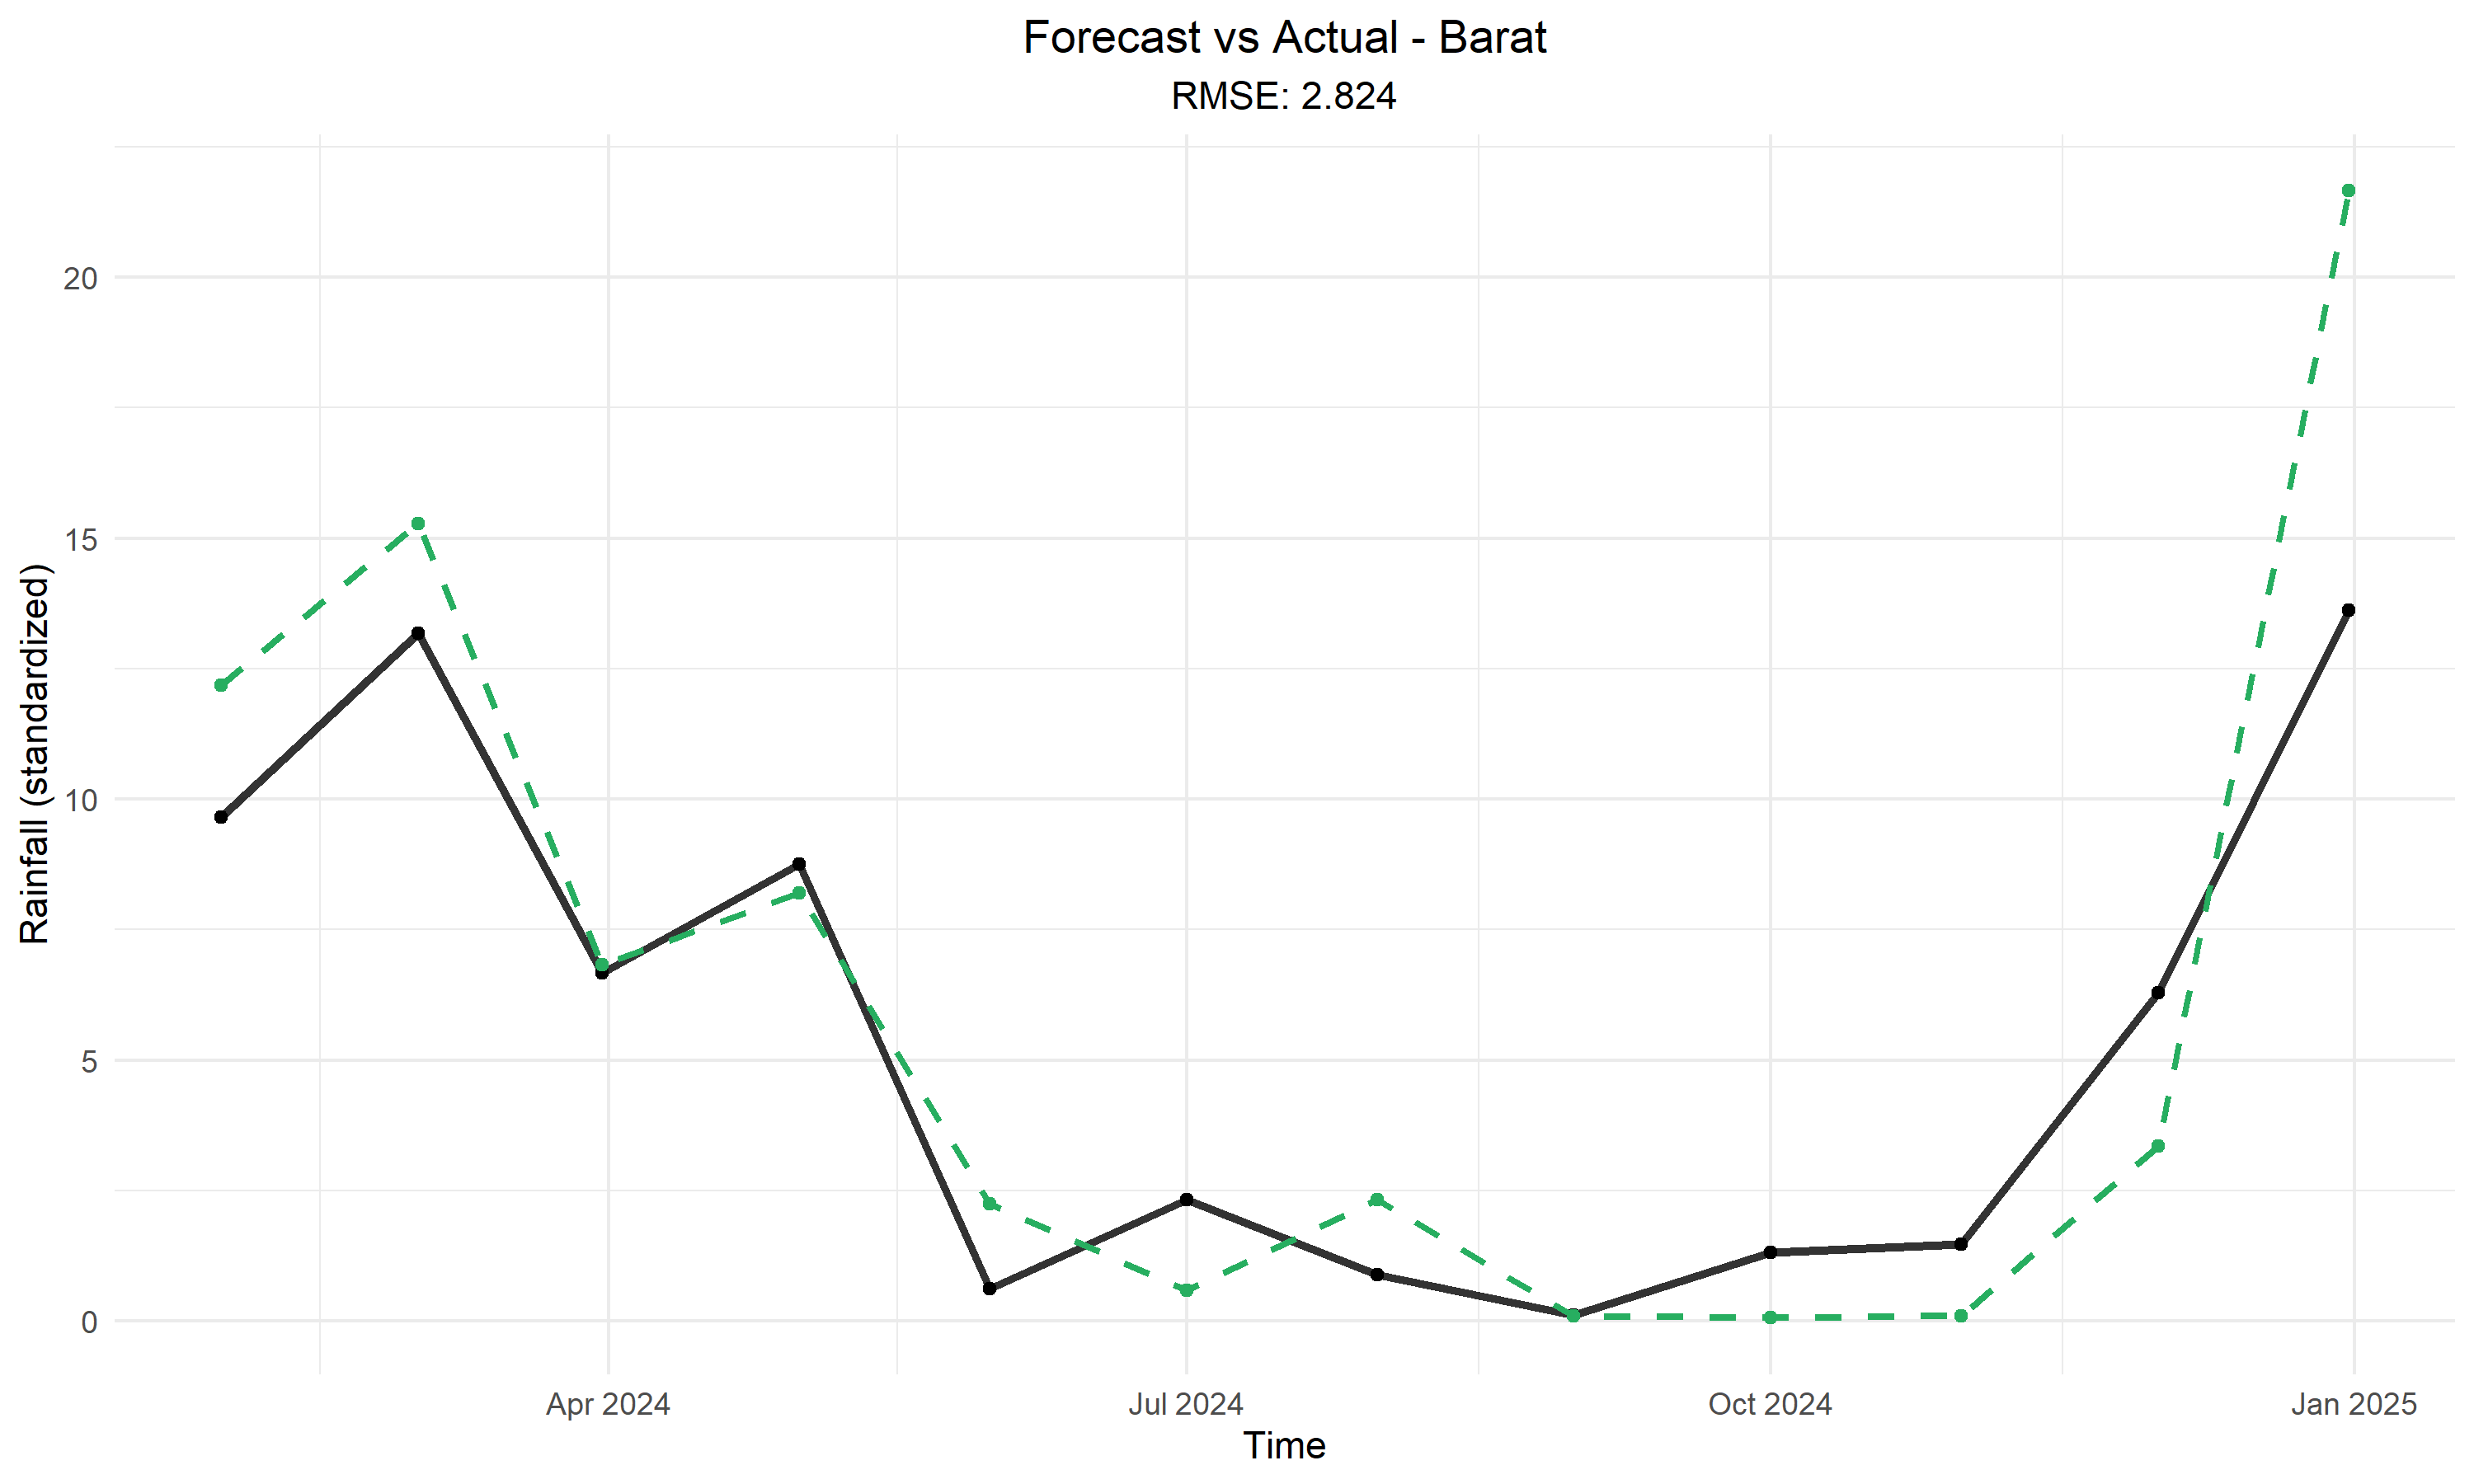
\includegraphics[width=0.9\textwidth]{images/bab_4/bab_4.3/bab_4.3.2/uniform-hasil-forecast-barat.png}
        \caption{Hasil Peramalan Wilayah Barat}
        \label{fig:starima-uniform-hasil-forecast-barat}
    \end{figure}
    Berdasarkan Gambar~\ref{fig:starima-uniform-hasil-forecast-barat} hasil prediksi curah hujan di Wilayah Barat menunjukkan nilai error sebesar 2,962, yang mengindikasikan bahwa tingkat kesalahan prediksi relatif kecil hingga menengah, sehingga model memiliki kemampuan peramalan yang cukup baik.
    Model mampu menangkap pola kenaikan curah hujan musiman di awal tahun dengan baik.
    Pada periode Mei hingga Agustus, terjadi penurunan curah hujan, dan hasil prediksi model masih mengikuti arah perubahan tersebut meskipun pada beberapa periode nilai prediksi sedikit lebih tinggi dibandingkan data aktual.
    Selanjutnya, mulai September hingga Desember, tren peningkatan curah hujan kembali terdeteksi dengan cukup akurat.
    Hal ini menunjukkan bahwa model mampu mengikuti dinamika perubahan curah hujan secara temporal dengan baik.
    \begin{figure}[H]
        \centering
        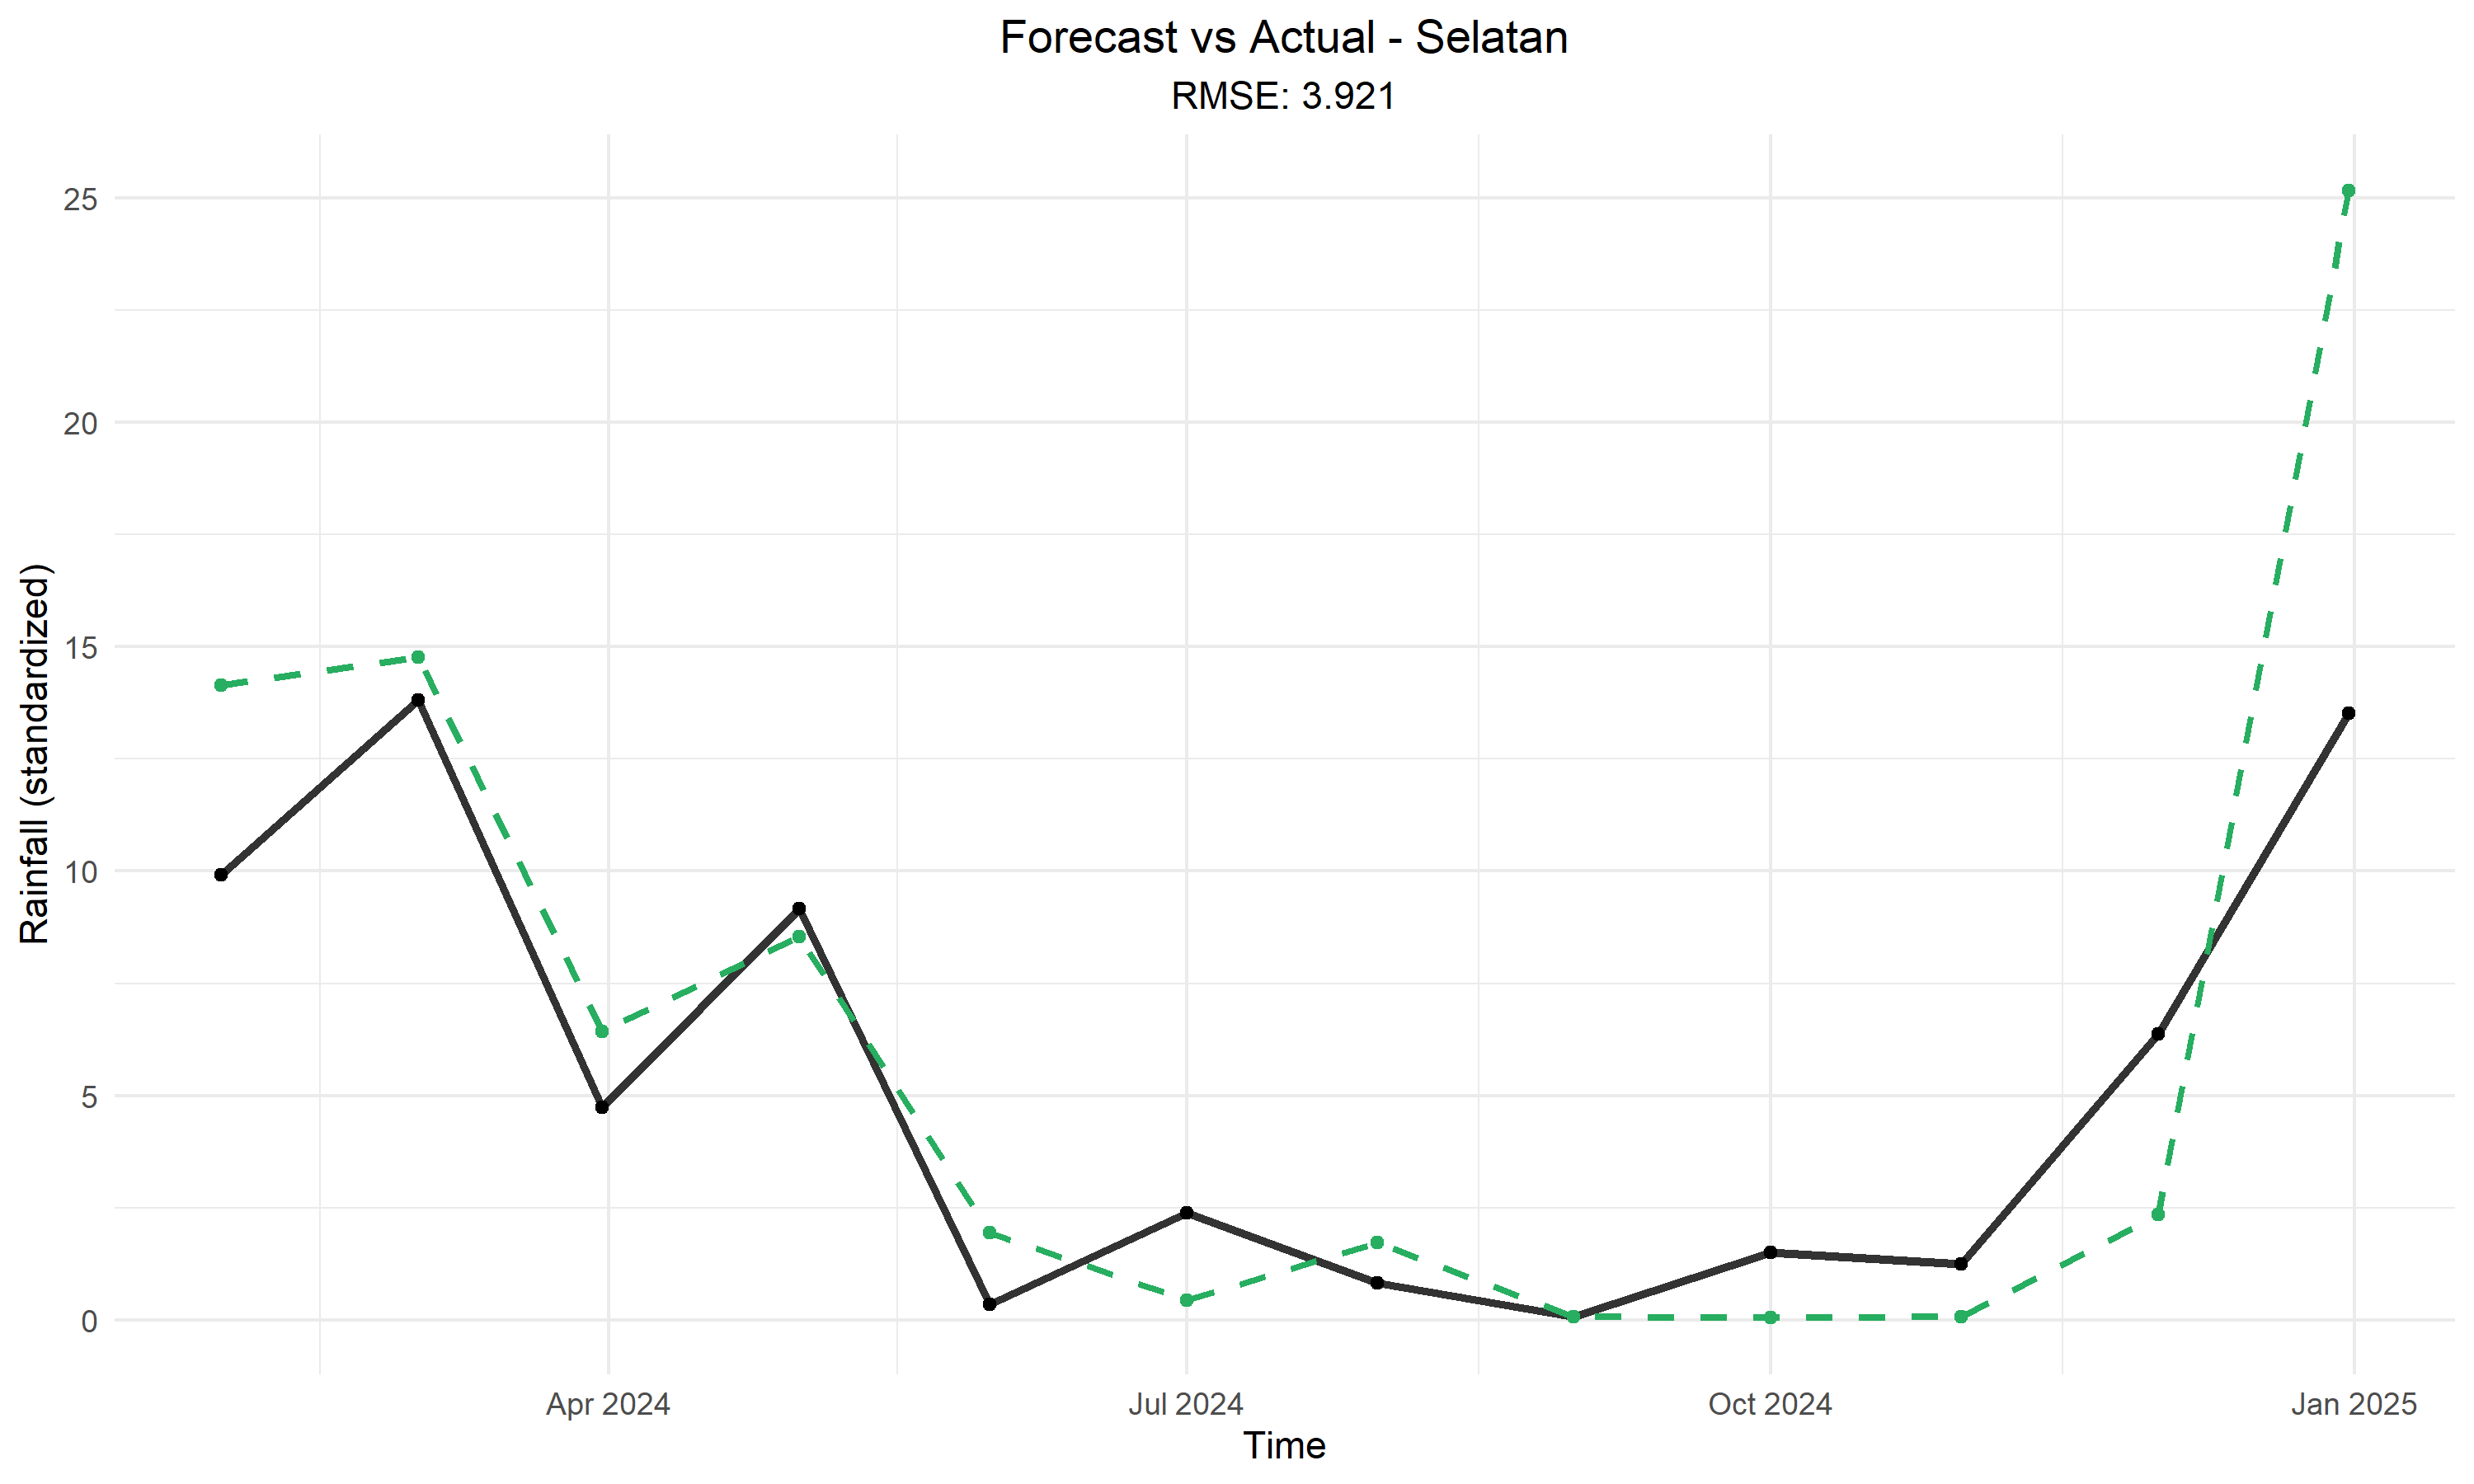
\includegraphics[width=0.9\textwidth]{images/bab_4/bab_4.3/bab_4.3.2/uniform-hasil-forecast-selatan.png}
        \caption{Hasil Peramalan Wilayah Selatan}
        \label{fig:starima-uniform-hasil-forecast-selatan}
    \end{figure}
    Berdasarkan Gambar~\ref{fig:starima-uniform-hasil-forecast-selatan} grafik menunjukkan bahwa model peramalan mampu menangkap pola musiman umum curah hujan di Wilayah Selatan dengan cukup baik, ditunjukkan oleh kemampuan model mengikuti penurunan curah hujan dari awal hingga pertengahan tahun serta kenaikan kembali menjelang akhir tahun.
    Pada periode curah hujan rendah (Juni–Oktober 2024), hasil prediksi relatif mendekati data aktual, menandakan kinerja model yang stabil pada kondisi tersebut.
    Namun, pada periode curah hujan tinggi di awal dan akhir tahun, model cenderung melakukan overestimate yang signifikan, terutama menjelang Januari 2025, sehingga berkontribusi terhadap nilai RMSE sebesar 3,921 yang tergolong cukup tinggi.
    Hal ini menunjukkan bahwa meskipun model efektif dalam menangkap tren dan musim, akurasinya masih terbatas dalam memprediksi lonjakan ekstrem curah hujan.
    \begin{figure}[H]
        \centering
        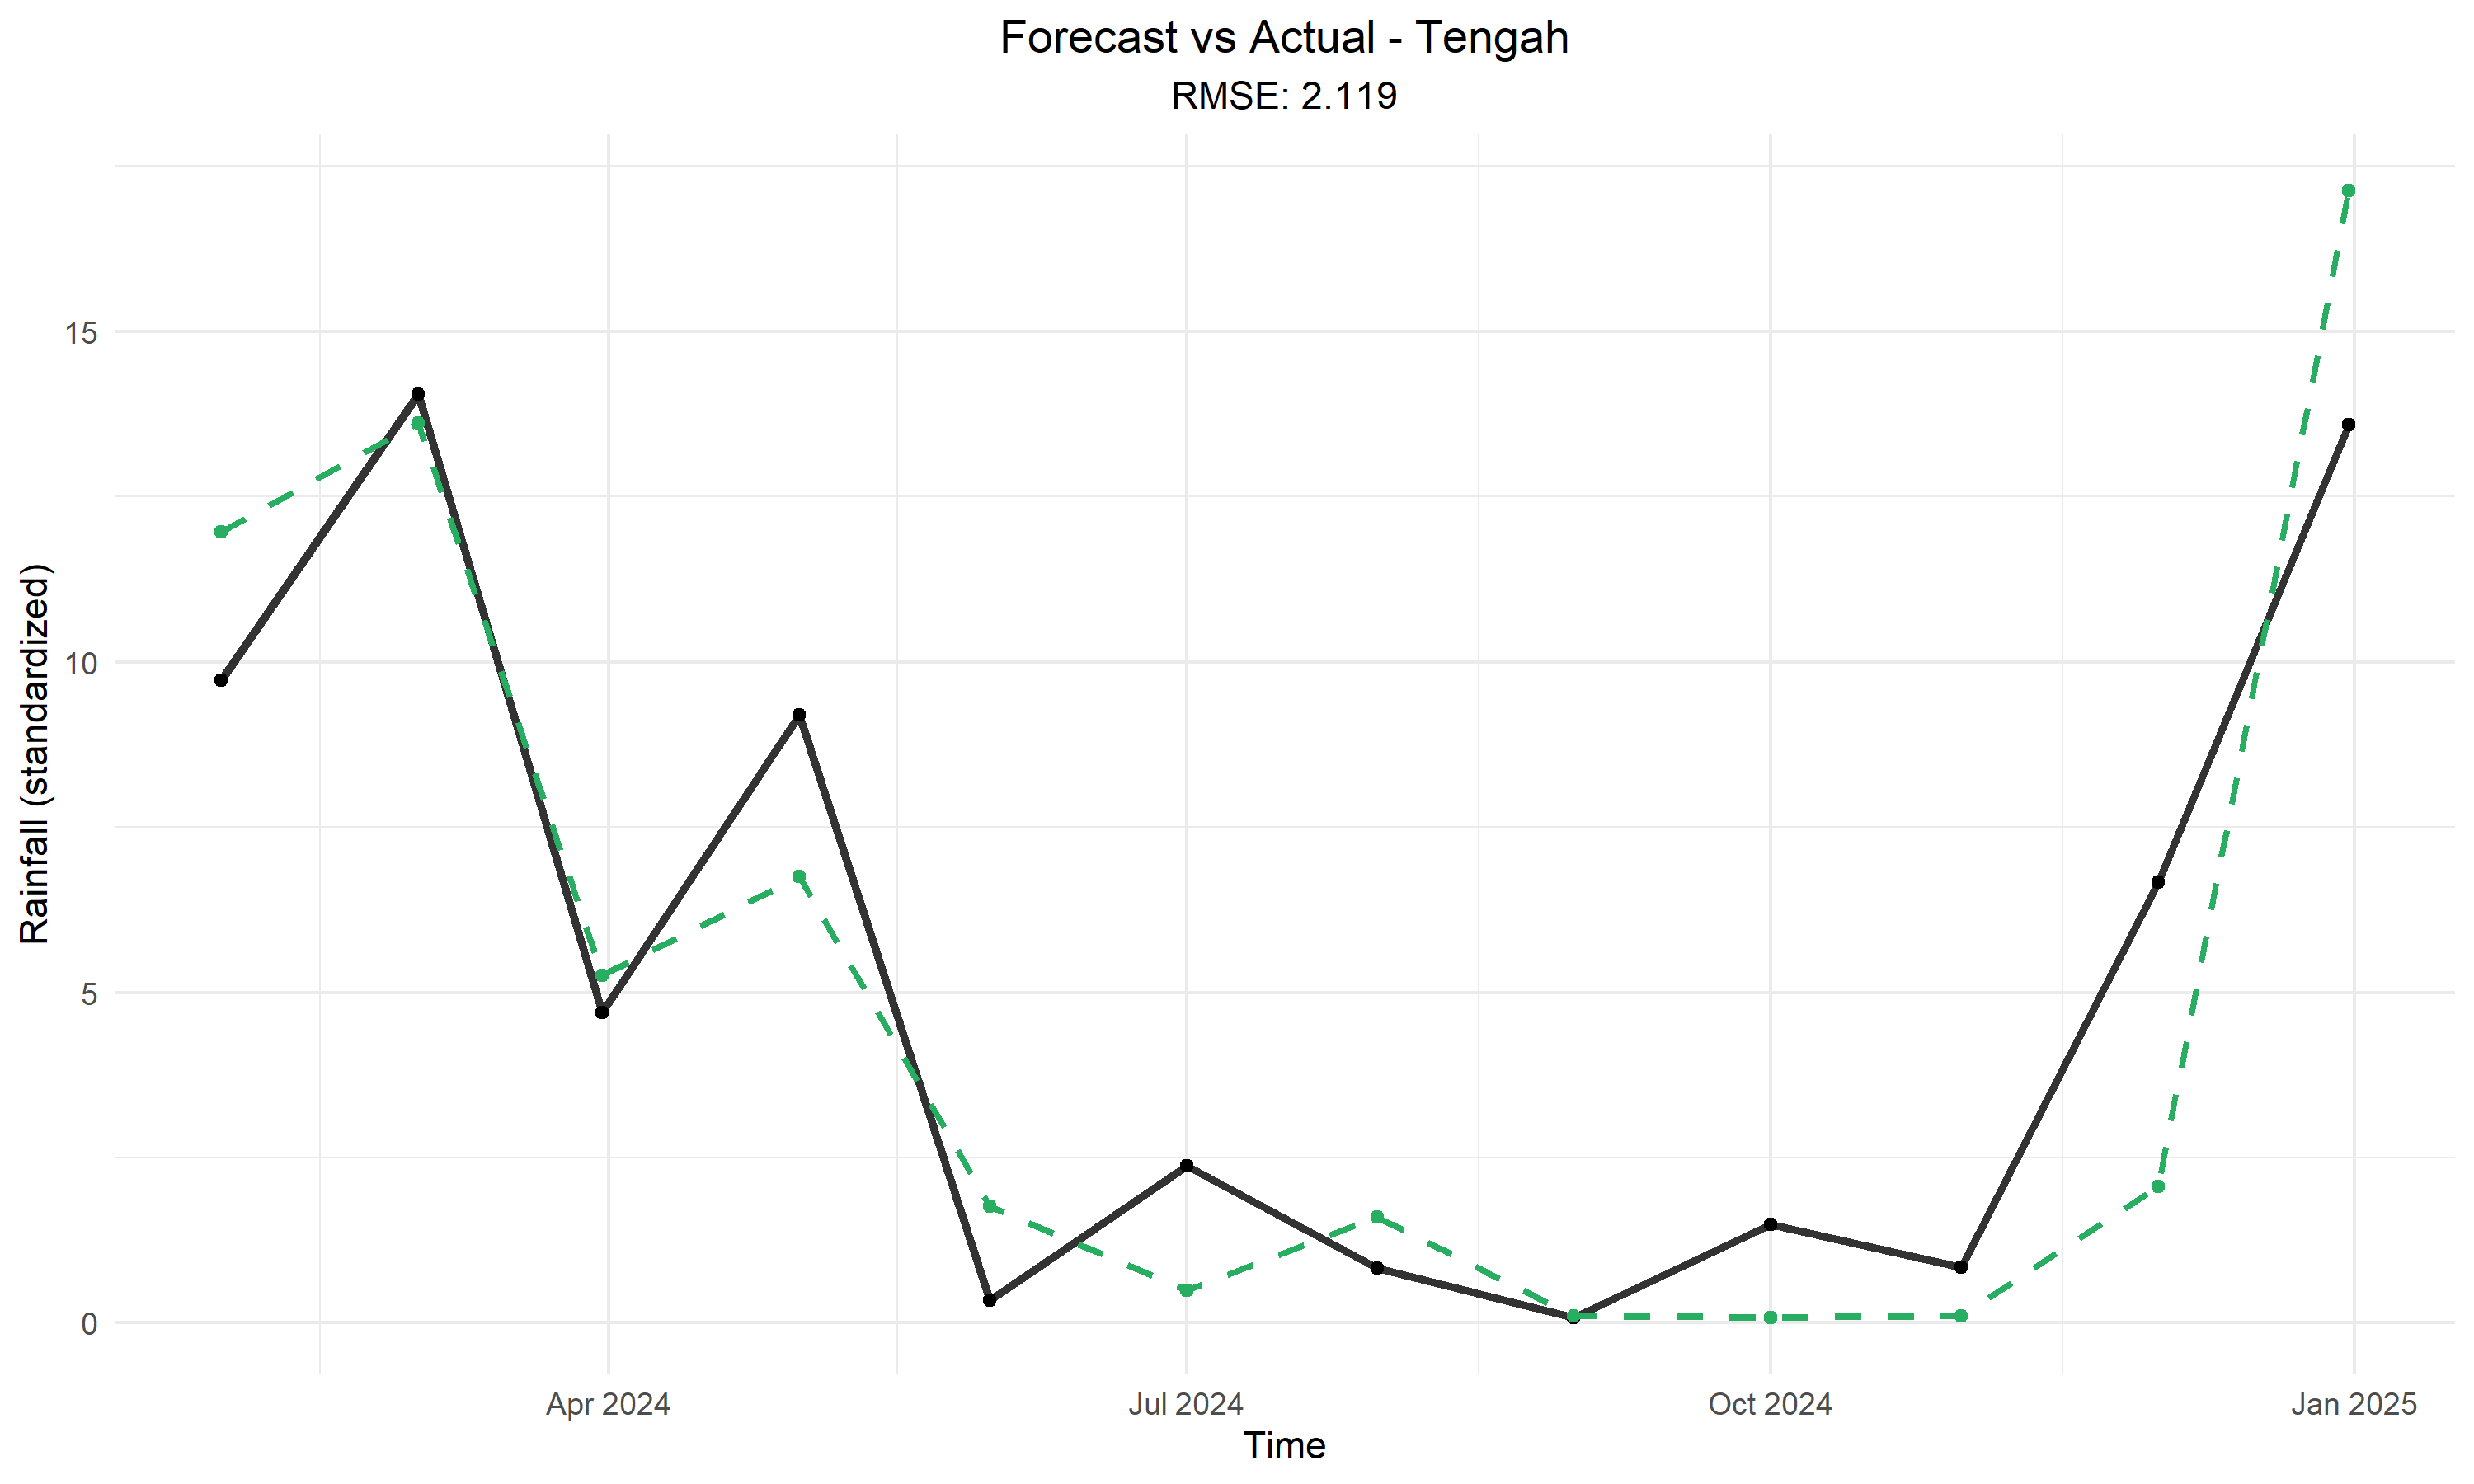
\includegraphics[width=0.9\textwidth]{images/bab_4/bab_4.3/bab_4.3.2/uniform-hasil-forecast-tengah.png}
        \caption{Hasil Peramalan Wilayah Tengah}
        \label{fig:starima-uniform-hasil-forecast-tengah}
    \end{figure}
    Berdasarkan Gambar~\ref{fig:starima-uniform-hasil-forecast-tengah} grafik menunjukkan bahwa model peramalan mampu mengikuti pola fluktuasi dan tren umum curah hujan di Wilayah Tengah dengan cukup baik, terutama pada periode awal hingga pertengahan tahun.
    Pada kondisi curah hujan rendah di pertengahan tahun, hasil prediksi relatif mendekati data aktual, menandakan kinerja model yang stabil.
    Namun, pada periode ekstrem di akhir tahun, khususnya menjelang Januari 2025, model cenderung melakukan overestimate, sehingga menurunkan akurasi prediksi.
    Nilai RMSE sebesar 4,092 menunjukkan tingkat kesalahan yang masih moderat, yang mengindikasikan bahwa model cukup baik dalam menangkap pola umum, tetapi masih memiliki keterbatasan dalam memprediksi lonjakan curah hujan ekstrem di Wilayah Tengah.
    \begin{figure}[H]
        \centering
        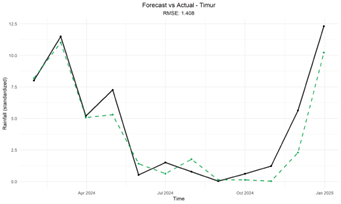
\includegraphics[width=0.9\textwidth]{images/bab_4/bab_4.3/bab_4.3.2/uniform-hasil-forecast-timur.png}
        \caption{Hasil Peramalan Wilayah Timur}
        \label{fig:starima-uniform-hasil-forecast-timur}
    \end{figure}
    Berdasarkan Gambar~\ref{fig:starima-uniform-hasil-forecast-timur} Grafik menunjukkan bahwa model peramalan memiliki kinerja sangat baik di Wilayah Timur, dengan nilai RMSE sebesar 1,331 yang tergolong rendah.
    Hasil prediksi terlihat sangat berdekatan dengan data aktual pada hampir seluruh periode pengamatan, baik pada kondisi curah hujan tinggi, rendah, maupun saat terjadi peningkatan kembali di akhir tahun.
    Model juga menunjukkan stabilitas tinggi tanpa deviasi ekstrem, serta mampu memprediksi kondisi curah hujan minimum dengan sangat akurat.
    Secara keseluruhan, hasil ini mengindikasikan bahwa model paling akurat dan konsisten dalam merepresentasikan dinamika curah hujan di Wilayah Timur dibandingkan wilayah lainnya.
    \begin{figure}[H]
        \centering
        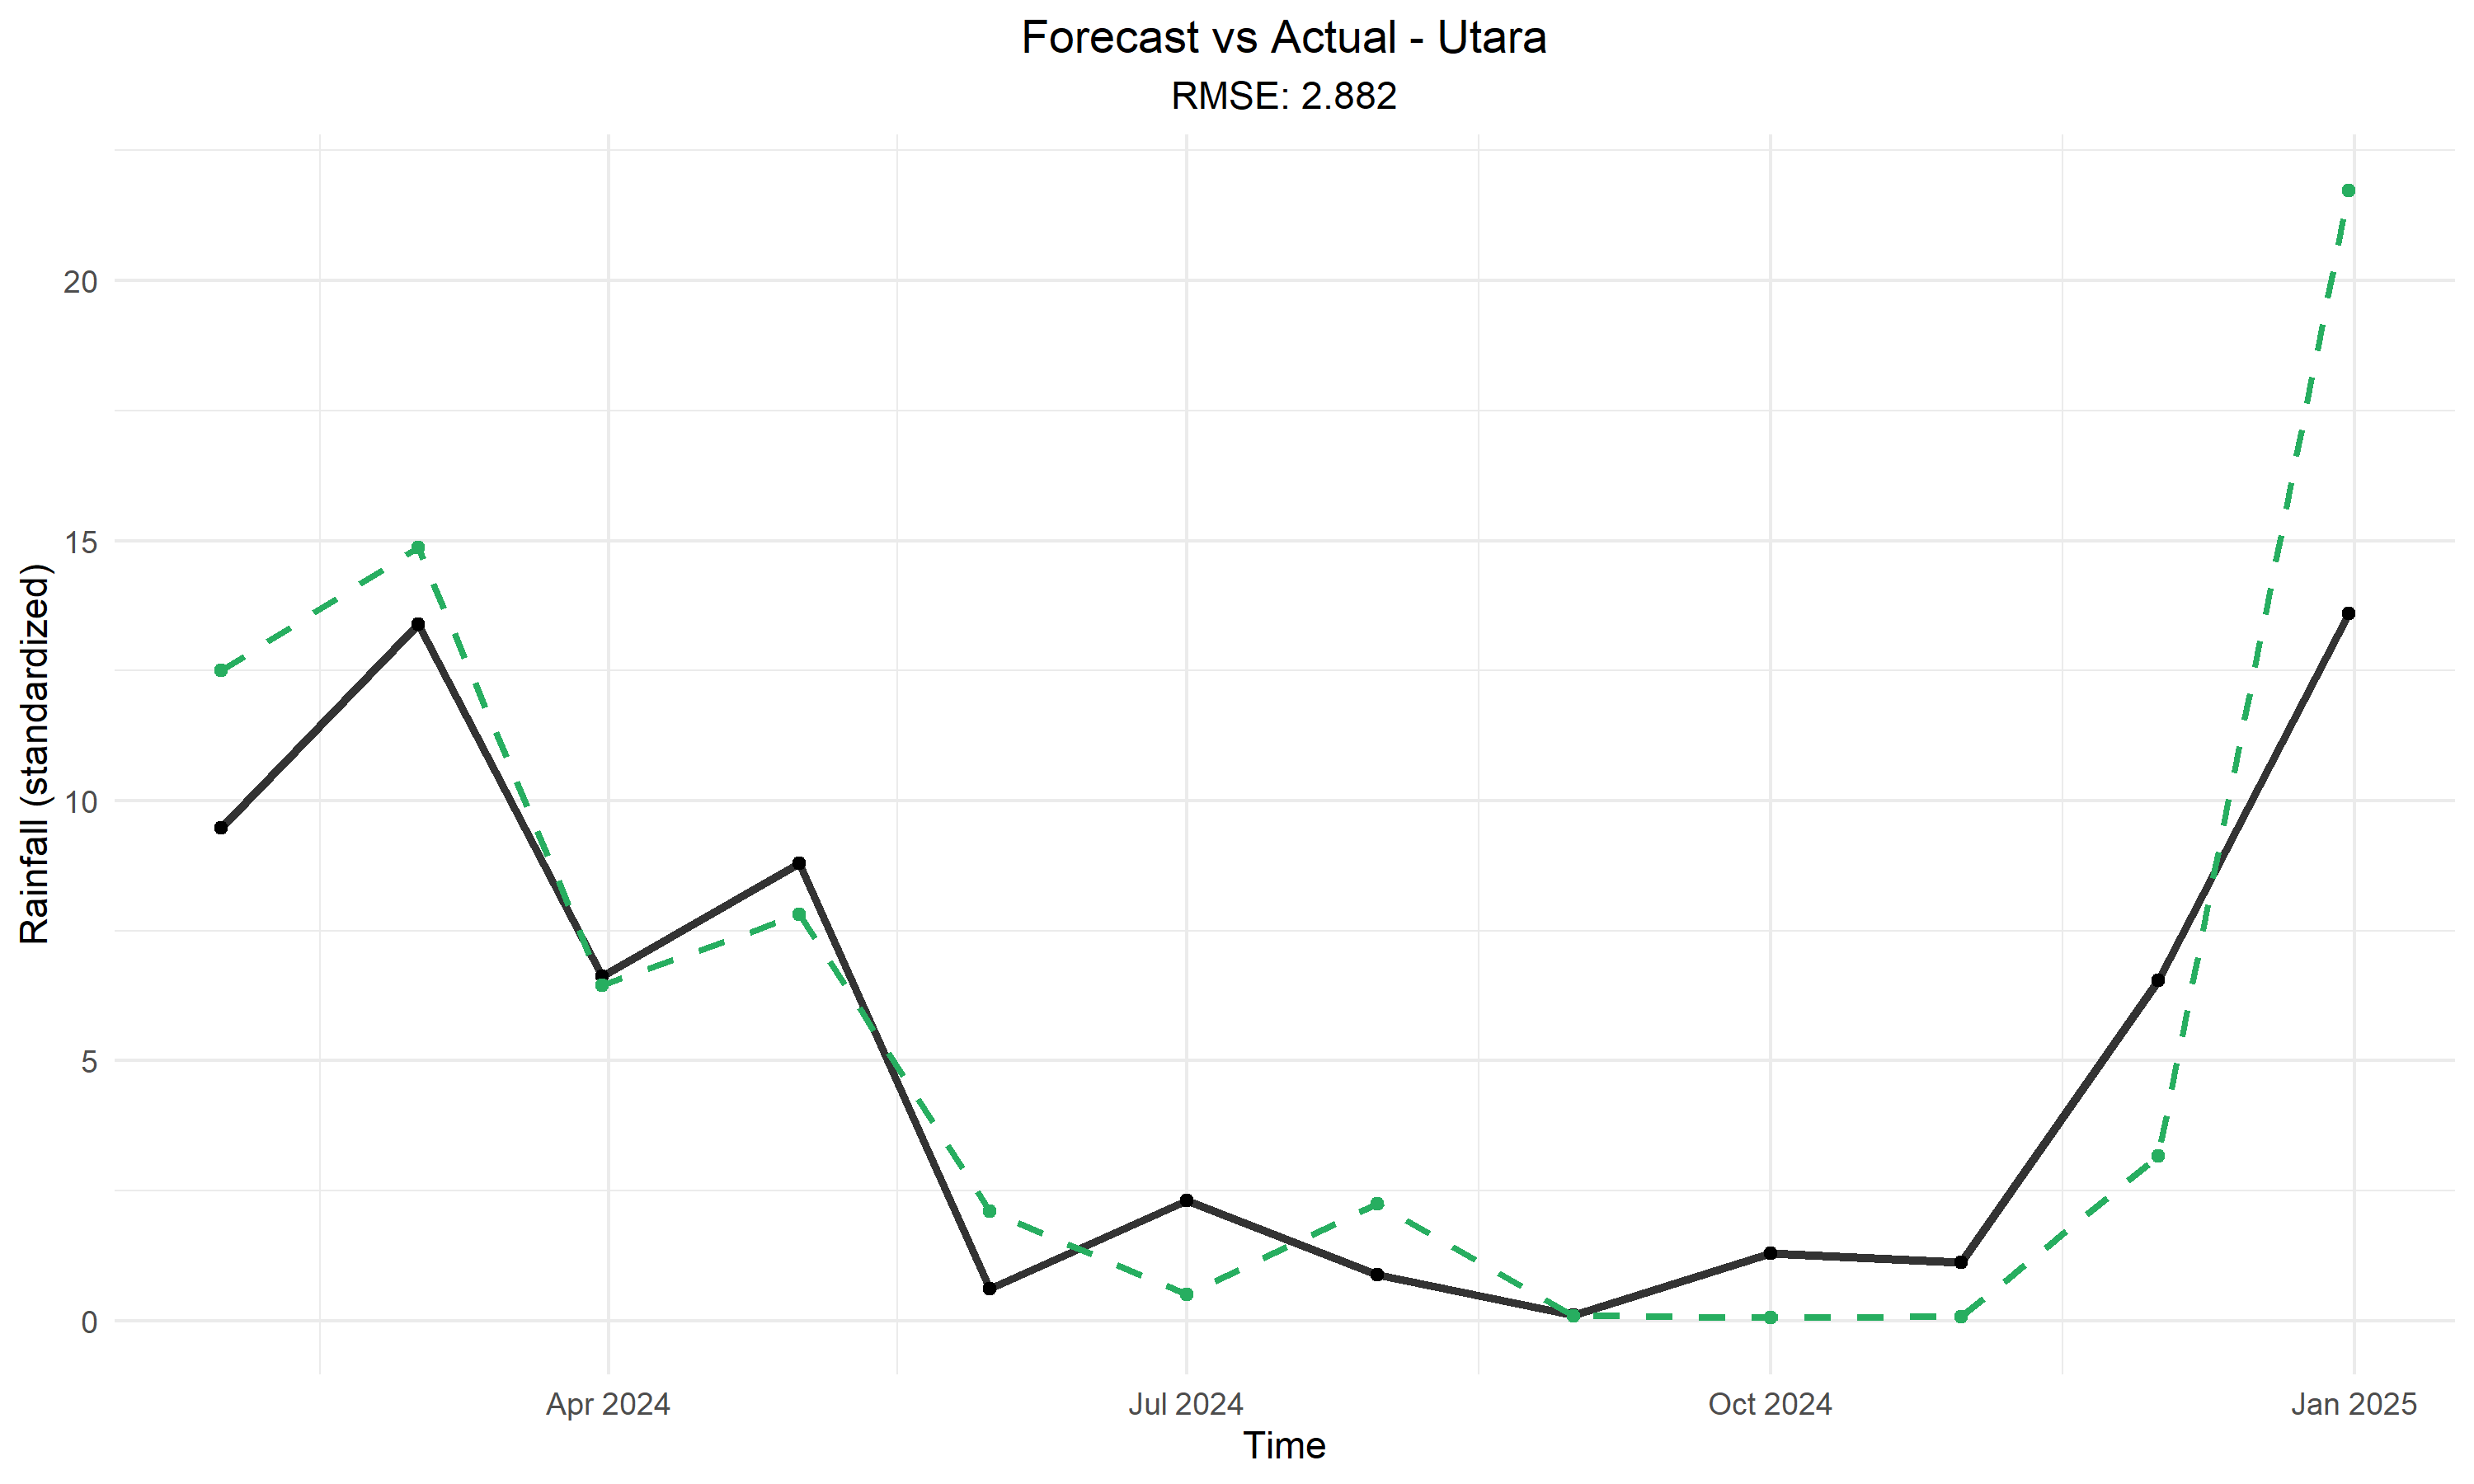
\includegraphics[width=0.9\textwidth]{images/bab_4/bab_4.3/bab_4.3.2/uniform-hasil-forecast-utara.png}
        \caption{Hasil Peramalan Wilayah Utara}
        \label{fig:starima-uniform-hasil-forecast-utara}
    \end{figure}
    Berdasarkan Gambar~\ref{fig:starima-uniform-hasil-forecast-utara} grafik menunjukkan bahwa model peramalan mampu mengikuti pola fluktuasi umum curah hujan di Wilayah Utara dengan cukup baik, termasuk penurunan di pertengahan tahun dan peningkatan menjelang akhir periode.
    Pada kondisi curah hujan rendah hingga sedang, hasil prediksi relatif mendekati data aktual, menandakan kinerja model yang stabil.
    Namun, pada periode ekstrem di akhir tahun, model cenderung melakukan overestimate, sehingga menurunkan akurasi prediksi.
    Nilai RMSE sebesar 2,922 menunjukkan tingkat kesalahan menengah, dengan akurasi yang lebih baik dibandingkan Wilayah Tengah, tetapi masih di bawah Wilayah Timur.
\end{enumerate}
\subsection{Bobot Invers Jarak}
Perhitungan bobot lokasi invers jarak menggunakan jarak sebenarnya antar lokasi, perhitungan bobot ini diperoleh dari hasil invers jarak sebenarnya yang kemudian dinormalisasi.
Perhitungan jarak antar wilayah dapat dilakukan sesuai dengan Persamaan~\ref{swm_inverse} yaitu dengan menggunakan posisi longitude dan latitude dari kedua wilayah yang akan dihitung jaraknya.
Posisi longitude dan latitude yang digunakan berupa jarak terluar atau terjauh dari masing masing wilayah Surabaya.
Bobot lokasi invers jarak memberikan nilai koefisien yang kecil untuk jarak yang lebih jauh dan sebaliknya.
Berikut merupakan matriks bobot lokasi invers jarak:
\begin{equation}
    \label{swm-bobot-inverse}
    W = 
    \begin{pmatrix}
        0.00 & 0.2380 & 0.2946 & 0.1612 & 0.3063 \\
        0.1896 & 0.00 & 0.3409 & 0.2637 & 0.2058 \\
        0.1727 & 0.2508 & 0.00 & 0.2031 & 0.3734 \\
        0.1482 & 0.3403 & 0.3186 & 0.00 & 0.2290 \\
        0.2112 & 0.1781 & 0.4910 & 0.1717 & 0.00 \\
    \end{pmatrix}
\end{equation}
\begin{enumerate}[label=\Alph*.]
    \item Identifikasi \\
    Setelah mendapatkan bobot, melakukan perhitungan STACF seperti pada Rumus~\ref{st_ma} dan STPACF seperti pada Rumus~\ref{st_ar}.
    Perhitungan Perthitungan STACF dan STPACF ini digunakan untuk menentukan orde $p$, $q$ nya karena data nya sudah di differencing.
    Berikut adalah plot STACF dan STPACF:
    \begin{figure}[H]
        \centering
        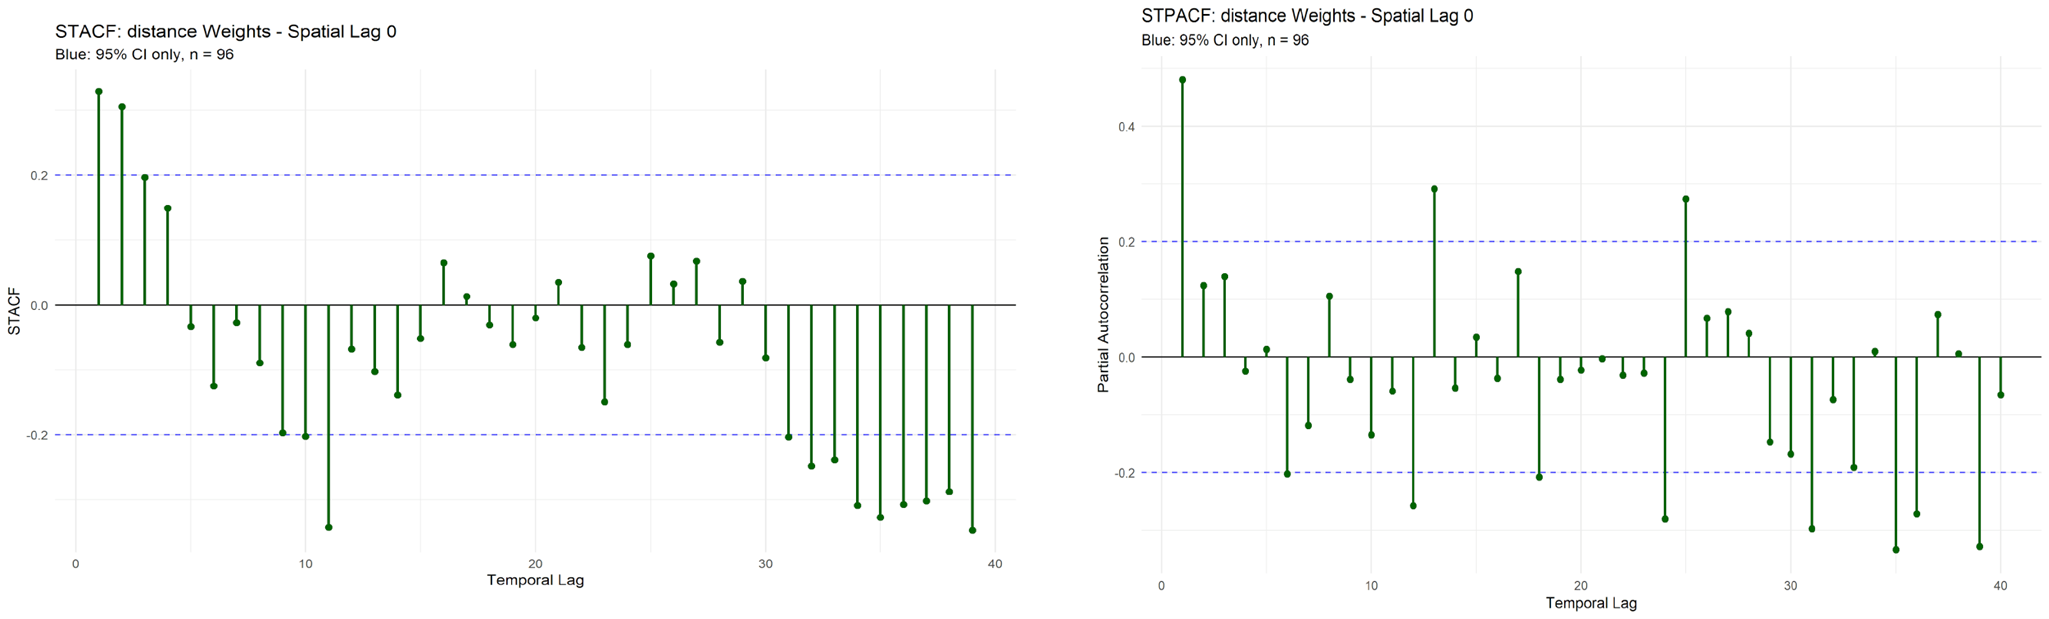
\includegraphics[width=0.9\textwidth]{images/bab_4/bab_4.3/bab_4.3.3/slag-0.png}
        \caption{STACF dan STPACF SLAG 0}
        \label{fig:slag-0-inverse}
    \end{figure}
    Gambar~\ref{fig:slag-0-inverse} menunjukkan hasil analisis \textit{Spatio-Temporal Autocorrelation Function} (STACF) dan \textit{Spatio Temporal Partial Autocorrelation Function} (STPACF) menggunakan invers jarak.
    Plot STACF menunjukkan adanya korelasi temporal jangka pendek serta pola musiman yang kuat pada lag ke-12 dan kelipatannya, yang mengindikasikan keberadaan komponen musiman tahunan.
    Sementara itu, plot STPACF menampilkan spike signifikan pada lag pertama dan lag musiman, yang mengarah pada keberadaan komponen autoregressive baik pada bagian non-musiman maupun musiman.
    Berdasarkan pola tersebut, model STARIMA dengan orde rendah pada komponen AR dan MA serta satu komponen musiman tahunan dinilai sesuai untuk memodelkan data.
    \begin{figure}[H]
        \centering
        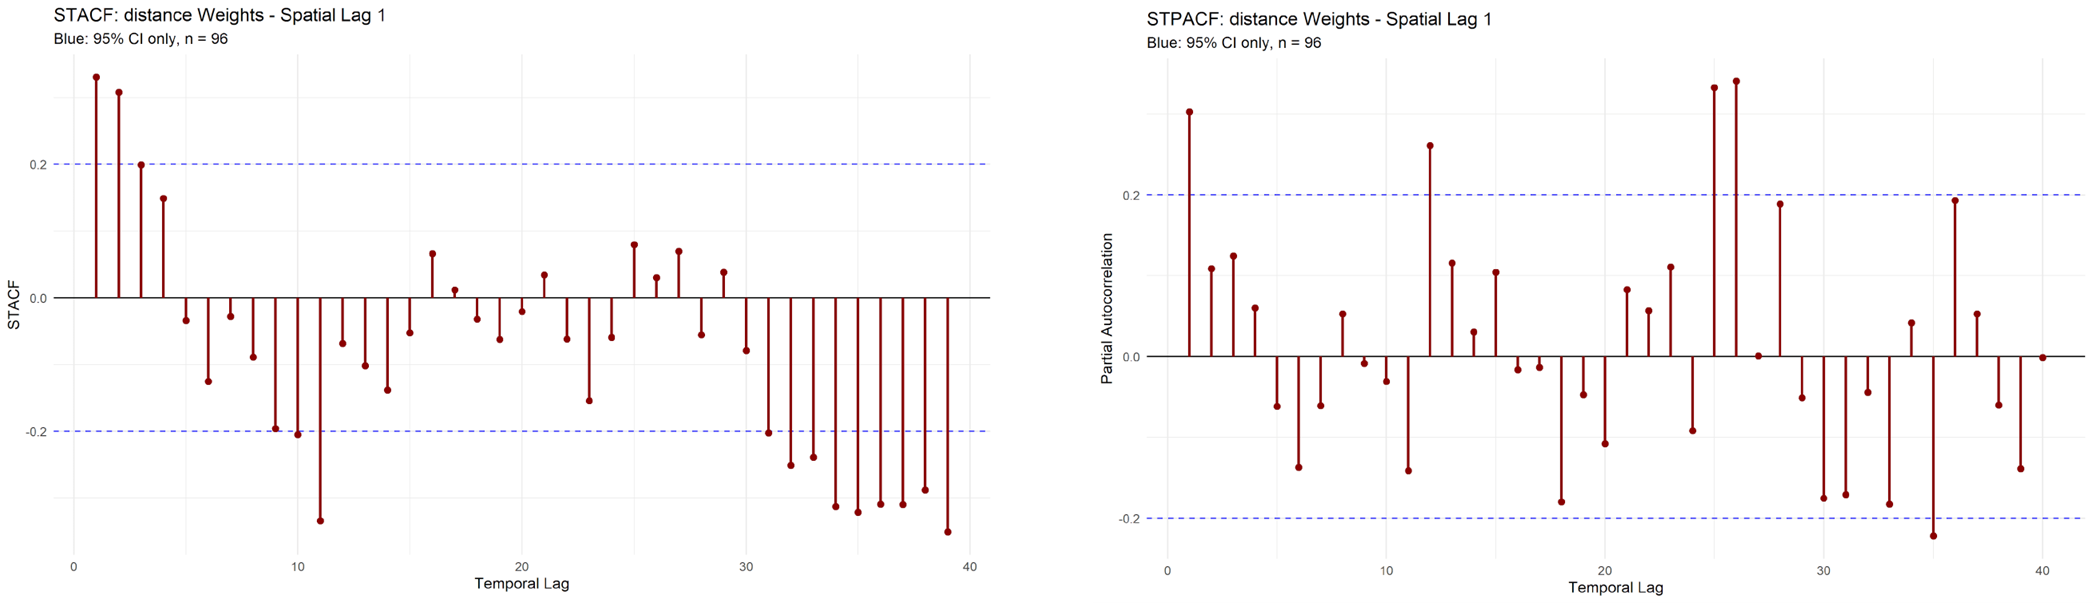
\includegraphics[width=0.9\textwidth]{images/bab_4/bab_4.3/bab_4.3.3/slag-1.png}
        \caption{STACF dan STPACF SLAG 1}
        \label{fig:slag-1-inverse}
    \end{figure}
    Gambar~\ref{fig:slag-1-inverse} menunjukkan hasil analisis \textit{Spatio Temporal Autocorrelation Function} (STACF) dan \textit{Spatio Temporal Partial Autocorrelation} (STPACF) menggunakan invers jarak.
    Plot STACF dan STPACF pada pembobot inverse jarak dengan spatial lag 1 menunjukkan pola korelasi yang tidak stabil dan tidak memberikan indikasi orde AR maupun MA yang jelas.
    Meskipun pola musiman tahunan masih terlihat, penambahan spatial lag 1 cenderung mengaburkan struktur temporal data.
    Hal ini menyebabkan parameter model STARIMA pada SLAG 1 tidak signifikan secara statistik, sehingga model dengan spatial lag 0 lebih layak digunakan.
    \item Estimasi Parameter \\
    Parameter yang diestimasi dari model yang telah diidentifikasi yaitu STARIMA $(0,0,1)(1,1,1)_{12}$ dan STARIMA $(0,0,0)(0,1,1_{0})_{12}$ menggunakan metode Maximum Likelihood, disajikan dalam Tabel~\ref{table:estimasi-paramater-starima-inverse}, bersama dengan standar error, nilai $t$, dan nilai $p$ masing-masing:
    \begin{table}[H]
    \centering
    \scriptsize
    \caption{Estimasi Parameter}
    \label{table:estimasi-paramater-starima-inverse}
    \renewcommand{\arraystretch}{1.25}

    \resizebox{\textwidth}{!}{
        \begin{tabular}{|c|c|c|c|c|c|c|c|c|}
            \hline
            \multirow{2}{*}{\textbf{Spatial Orde}} &
            \multirow{2}{*}{\textbf{Model}} &
            \multirow{2}{*}{\textbf{Statistik}} &
            \multicolumn{3}{c|}{\textbf{AR Parameter}} &
            \multicolumn{3}{c|}{\textbf{MA Parameter}} \\ \cline{4-9}

            & & &
            \multicolumn{1}{c|}{$\phi_{10}$} &
            \multicolumn{1}{c|}{$\Phi_{20}$} &
            \multicolumn{1}{c|}{$\Phi_{30}$} &
            \multicolumn{1}{c|}{$\Theta_{10}$} &
            \multicolumn{1}{c|}{$\Theta_{20}$} &
            $\Theta_{30}$ \\ 
            \hline

            % ===================== LAG 0 ==========================
            \multirow{12}{*}{Lag 0}
            & \multirow{4}{*}{1,1,0}
            & Estimasi & 0.4812 &  &  &  &  &  \\ \cline{3-9}
            & & SE      & 0.0435 &  &  &  &  &  \\ \cline{3-9}
            & & t-value & 11.1   &  &  &  &  &  \\ \cline{3-9}
            & & p-value & $<0.0000000000000002$ *** &  &  &  &  &  \\ \cline{2-9}

            & \multirow{4}{*}{1,1,1}
            & Estimasi & 0.5747 &  &  & -0.1557 &  &  \\ \cline{3-9}
            & & SE      & 0.0685 &  &  & 0.0853 &  &  \\ \cline{3-9}
            & & t-value & 8.39   &  &  & -1.83  &  &  \\ \cline{3-9}
            & & p-value & 0.0000000000000056 *** & 0.069 &  &  &  &  \\ \cline{2-9}

            & \multirow{4}{*}{1,1,2}
            & Estimasi & 0.6760 & -0.2765 & -0.1313 &  &  &  \\ \cline{3-9}
            & & SE      & 0.088  & 0.1082 & 0.076  &  &  &  \\ \cline{3-9}
            & & t-value & 7.62   & 2.56   & 1.71   &  &  &  \\ \cline{3-9}
            & & p-value & 0.00000000000014 *** & 0.011 *** & 0.087 &  &  &  \\ 
            \hline

            % ===================== LAG 1 ==========================
            \multirow{12}{*}{Lag 1}
            & \multirow{4}{*}{1,1,0}
            & Estimasi & 0.4849 &  &  &  &  &  \\ \cline{3-9}
            & & SE      & 0.0436 &  &  &  &  &  \\ \cline{3-9}
            & & t-value & 11.1   &  &  &  &  &  \\ \cline{3-9}
            & & p-value & $<0.0000000000000002$ *** &  &  &  &  & \\ \cline{2-9}

            & \multirow{4}{*}{1,1,1}
            & Estimasi & 0.5694 &  &  & -0.1423 &  &  \\ \cline{3-9}
            & & SE      & 0.0682 &  &  & 0.0855 &  &  \\ \cline{3-9}
            & & t-value & 8.34   &  &  & 1.66  &  &  \\ \cline{3-9}
            & & p-value & 0.0000000000000078 *** & 0.097 &  &  &  & \\ \cline{2-9}

            & \multirow{4}{*}{1,1,2}
            & Estimasi & 0.6760 & -0.2792 & -0.1297 &  &  &  \\ \cline{3-9}
            & & SE      & 0.1114 & 0.1385 & 0.0983 &  &  &  \\ \cline{3-9}
            & & t-value & 6.07   & -2.02  & -1.32  &  &  &  \\ \cline{3-9}
            & & p-value & 0.0000000026 *** & 0.044 & 0.187 &  &  & \\ 
            \hline

        \end{tabular}
    }
\end{table}
    Berdasarkan Tabel~\ref{table:estimasi-paramater-starima-inverse} hasil estimasi parameter dari kedua model dari lag spasial 0 dan lag spasial 1 yang di estimasi menggunakan metode Maximum Likelihood.
    Masing-masing parameter dilaporkan bersama standar error, nilai $t$, dan nilai $p$ untuk menilai signifikansi statistik.
    Secara umum berdasarkan signifikansi, model STARIMA dengan spatial lag 0 merupakan model terbaik. Model STARIMA $(0,0,1) x (1,1,1)_{12}$ dengan spatial lag 0 memiliki seluruh parameter yang signifikan dan mampu menangkap dinamika temporal jangka pendek serta pola musiman tahunan secara komprehensif.
    Sebaliknya, model STARIMA $(0,0,0) x (0,1,1_{0})_{12}$ dengan spatial lag 1 hanya menangkap komponen musiman dan menunjukkan struktur yang terlalu sederhana.
    Oleh karena itu, model dengan spatial lag 0 dinilai lebih layak digunakan sebagai model akhir dalam penelitian ini.

    \item Model Terbaik \\
    Untuk memilih model spasial terbaik dalam penelitian ini menggunakan evaluasi \textit{Root Mean Squared Error} (RMSE) untuk membandingkan kinerja peramalan dari model-model STARIMA. 
    Berdasarkan hasil pada Lampiran~\ref{lampiran:rmse-inverse},  berikut adalah tabel nya:
    \begin{table}[H]
    \centering
    \caption{Hasil Model Fitting STARIMA}
    \label{table:hasil-model-fitting-starima-inverse}
    \renewcommand{\arraystretch}{1.3}

    \resizebox{\textwidth}{!}{
        \begin{tabular}{lcccc}
            \toprule
            \textbf{Wilayah} &
            \textbf{STARIMA (1,1,0)\textsubscript{0}} &
            \textbf{STARIMA (1,1,1)\textsubscript{0}} &
            \textbf{STARIMA (1,1,0)\textsubscript{1}} &
            \textbf{STARIMA (1,1,1)\textsubscript{1}} \\
            \midrule

            Barat   & 1.688 & 1.652 & 1.686 & 1.653 \\
            Selatan & 2.020 & 2.005 & 2.020 & 2.005 \\
            Tengah  & 2.067 & 2.127 & 2.067 & 2.121 \\
            Timur   & 1.420 & 1.407 & 1.419 & 1.407 \\
            Utara   & 1.698 & 1.681 & 1.696 & 1.681 \\

            \midrule
            \textbf{Rata-Rata} & 1.7786 & 1.7744 & 1.7776 & 1.7734 \\
            \bottomrule
        \end{tabular}
    }
\end{table}
    Berdasarkan Tabel~\ref{table:hasil-model-fitting-starima-inverse}, terlihat bahwa evaluasi nilai RMSE per wilayah, model STARIMA $(0,0,1) x (1,1,1)_{12}$ menunjukkan kinerja yang lebih baik pada sebagian besar wilayah secara individual.
    Namun, ditinjau dari nilai RMSE rata-rata, model STARIMA $(0,0,0) x (0,1,1_{0})_{12}$ menghasilkan error yang lebih kecil secara keseluruhan.
    Dengan mempertimbangkan prinsip parsimoni dan kestabilan kinerja global, model STARIMA $(0,0,0) x (0,1,1_{0})_{12}$ dipilih sebagai model terbaik untuk peramalan curah hujan.

    \item Hasil Forecasting STARIMA
    Berikut adalah hasil peramalan curah hujan di berbagai wilayah menggunakan bobot invers jarak:
    \begin{figure}[H]
        \centering
        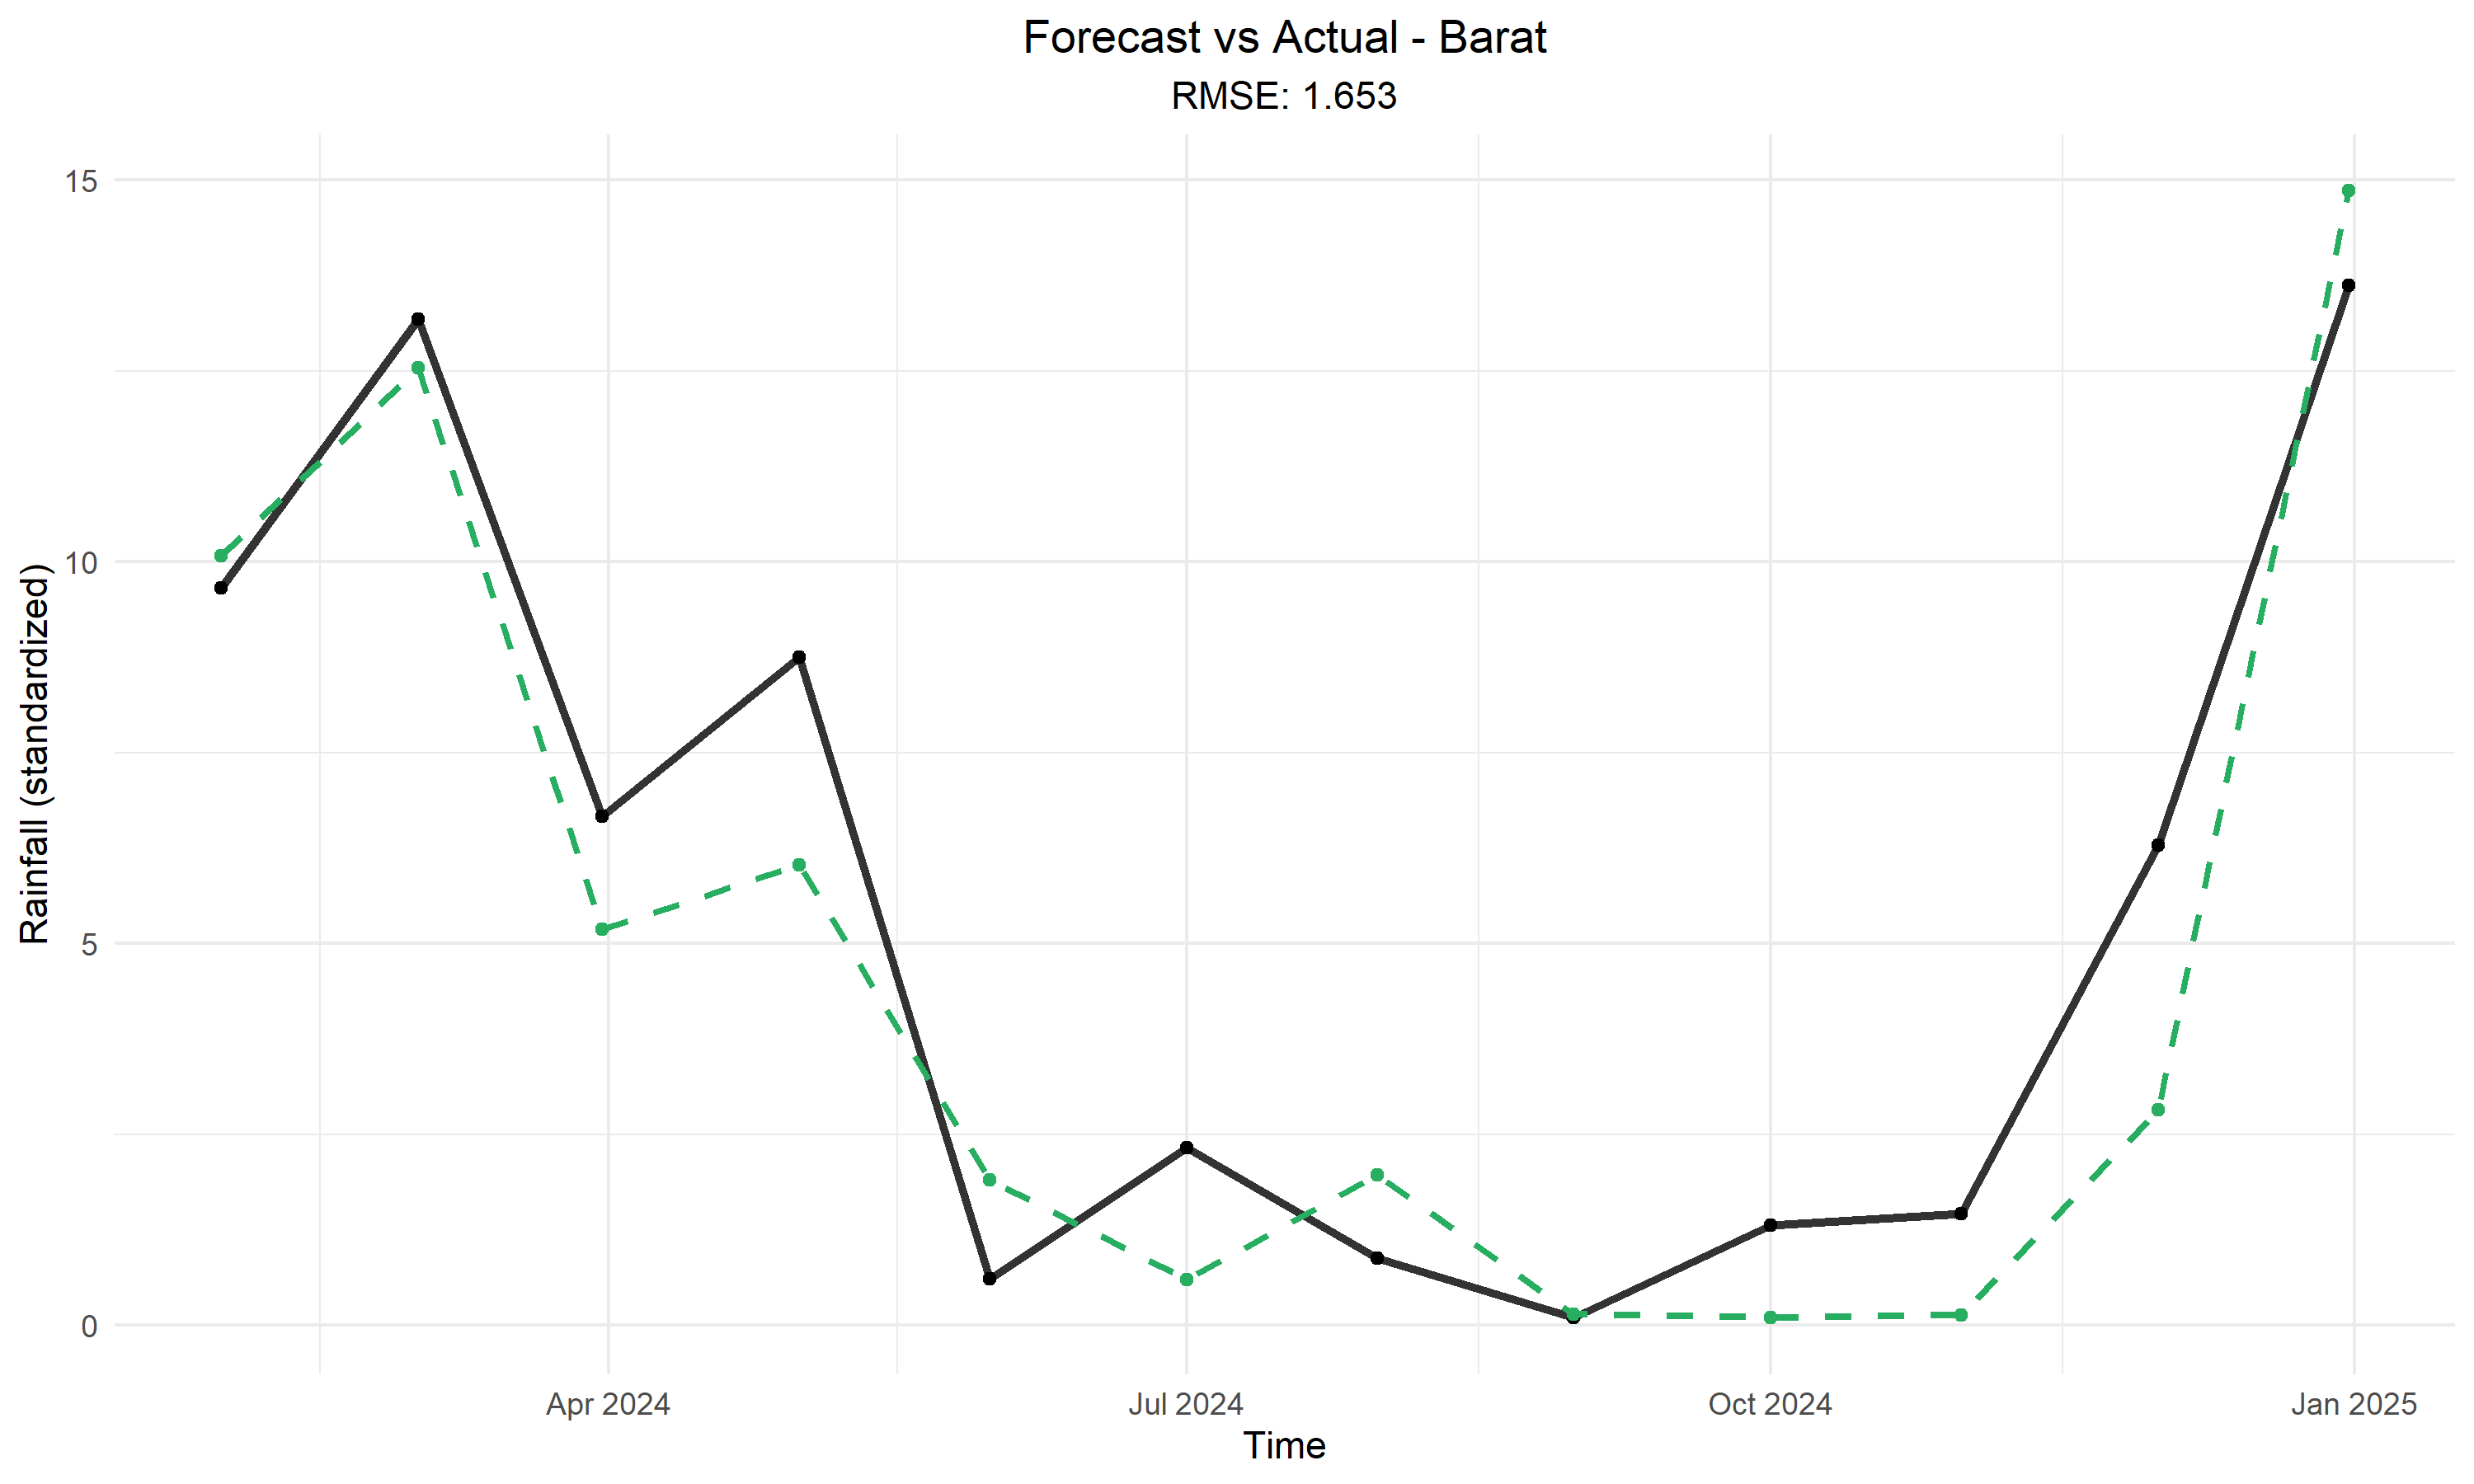
\includegraphics[width=0.9\textwidth]{images/bab_4/bab_4.3/bab_4.3.3/inverse-hasil-forecast-barat.png}
        \caption{Hasil Peramalan Wilayah Barat}
        \label{fig:starima-inverse-hasil-forecast-barat}
    \end{figure}
    Berdasarkan Gambar~\ref{fig:starima-inverse-hasil-forecast-barat} grafik menunjukkan bahwa model peramalan di Wilayah Barat memiliki kinerja cukup baik dengan nilai RMSE sebesar 2,753.
    Model mampu mengikuti pola naik-turun curah hujan secara umum, terutama pada awal periode dan saat curah hujan rendah di pertengahan tahun, di mana selisih antara nilai aktual dan ramalan relatif kecil.
    Namun, pada periode ekstrem di akhir tahun, model cenderung melakukan overestimate terhadap lonjakan curah hujan, sehingga akurasinya menurun.
    Secara keseluruhan, model layak digunakan untuk peramalan umum, tetapi masih memiliki keterbatasan dalam memprediksi kejadian curah hujan ekstrem.
    \begin{figure}[H]
        \centering
        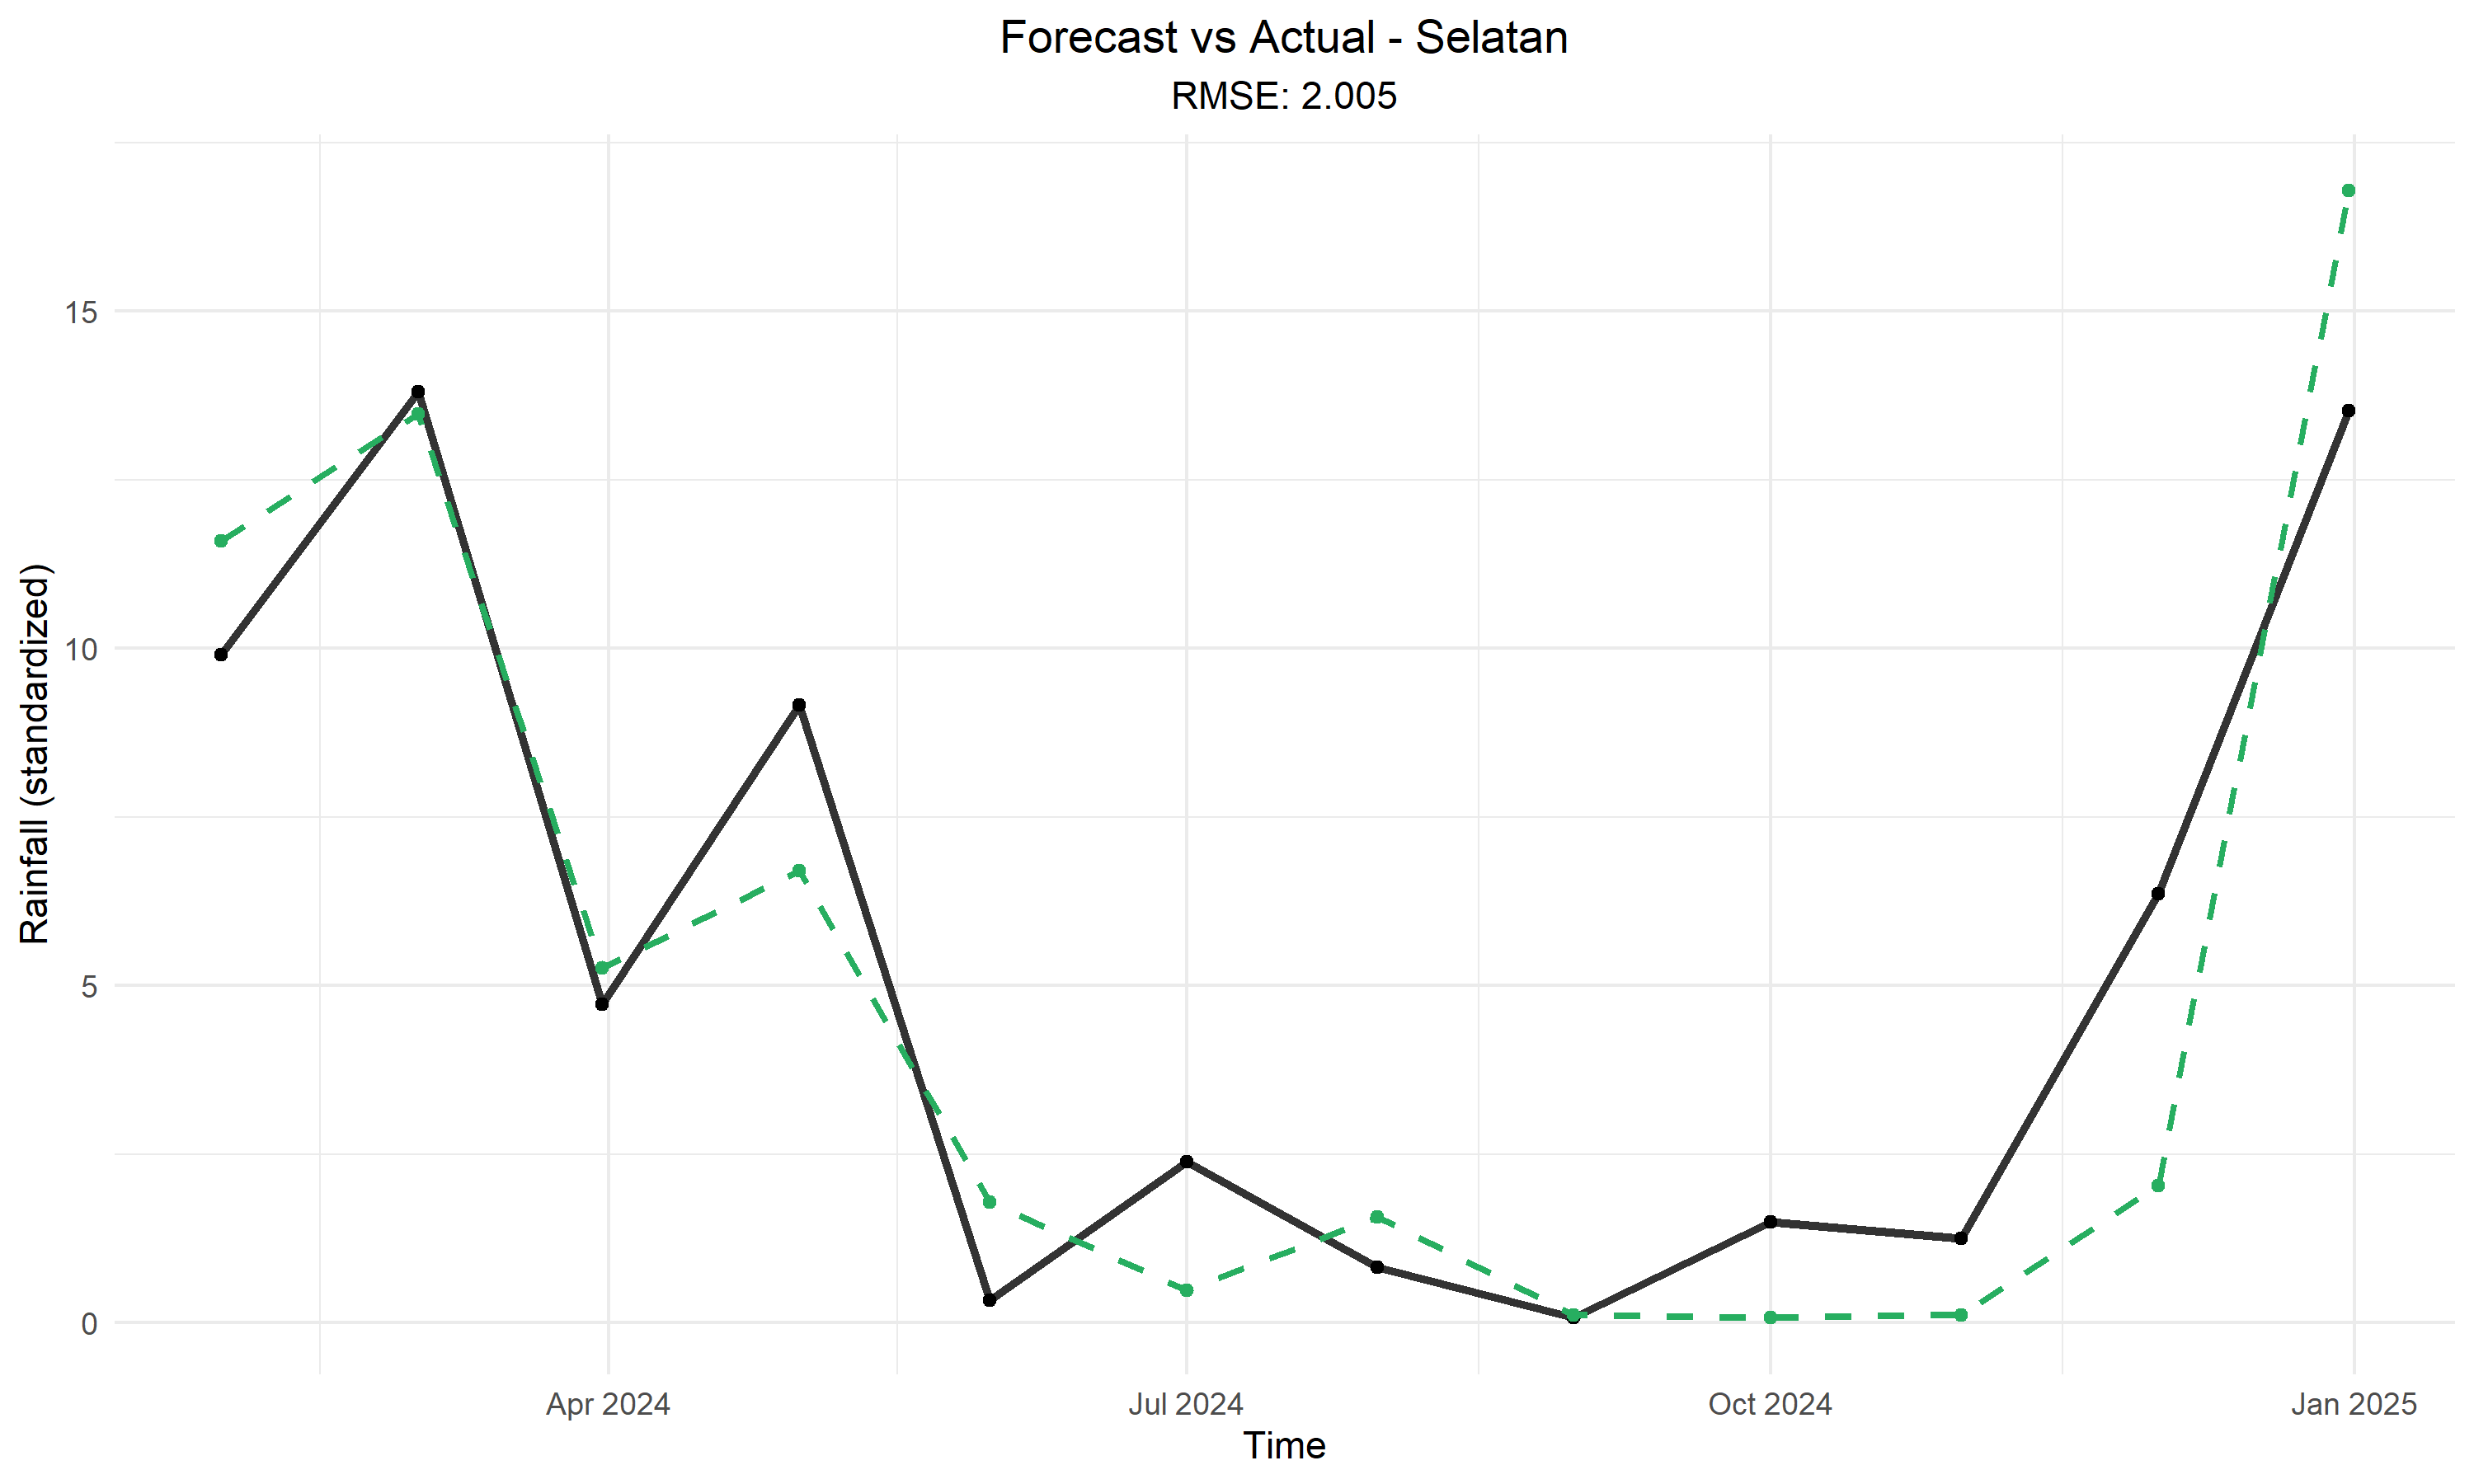
\includegraphics[width=0.9\textwidth]{images/bab_4/bab_4.3/bab_4.3.3/inverse-hasil-forecast-selatan.png}
        \caption{Hasil Peramalan Wilayah Selatan}
        \label{fig:starima-inverse-hasil-forecast-selatan}
    \end{figure}
    Berdasarkan Gambar~\ref{fig:starima-inverse-hasil-forecast-selatan} grafik menunjukkan bahwa model peramalan di Wilayah Selatan mampu menangkap pola musiman umum curah hujan dengan cukup baik, terutama pada awal hingga pertengahan periode.
    Pada kondisi curah hujan rendah hingga sedang, hasil prediksi relatif mendekati data aktual, menandakan kinerja model yang cukup andal.
    Namun, pada periode ekstrem di akhir tahun, model cenderung melakukan overestimate terhadap lonjakan curah hujan, sehingga meningkatkan nilai kesalahan prediksi.
    Nilai RMSE sebesar 3,667 menunjukkan bahwa akurasi model di Wilayah Selatan lebih rendah dibandingkan Wilayah Barat, yang mengindikasikan variabilitas curah hujan yang lebih tinggi dan keterbatasan model dalam memprediksi perubahan ekstrem.
    \begin{figure}[H]
        \centering
        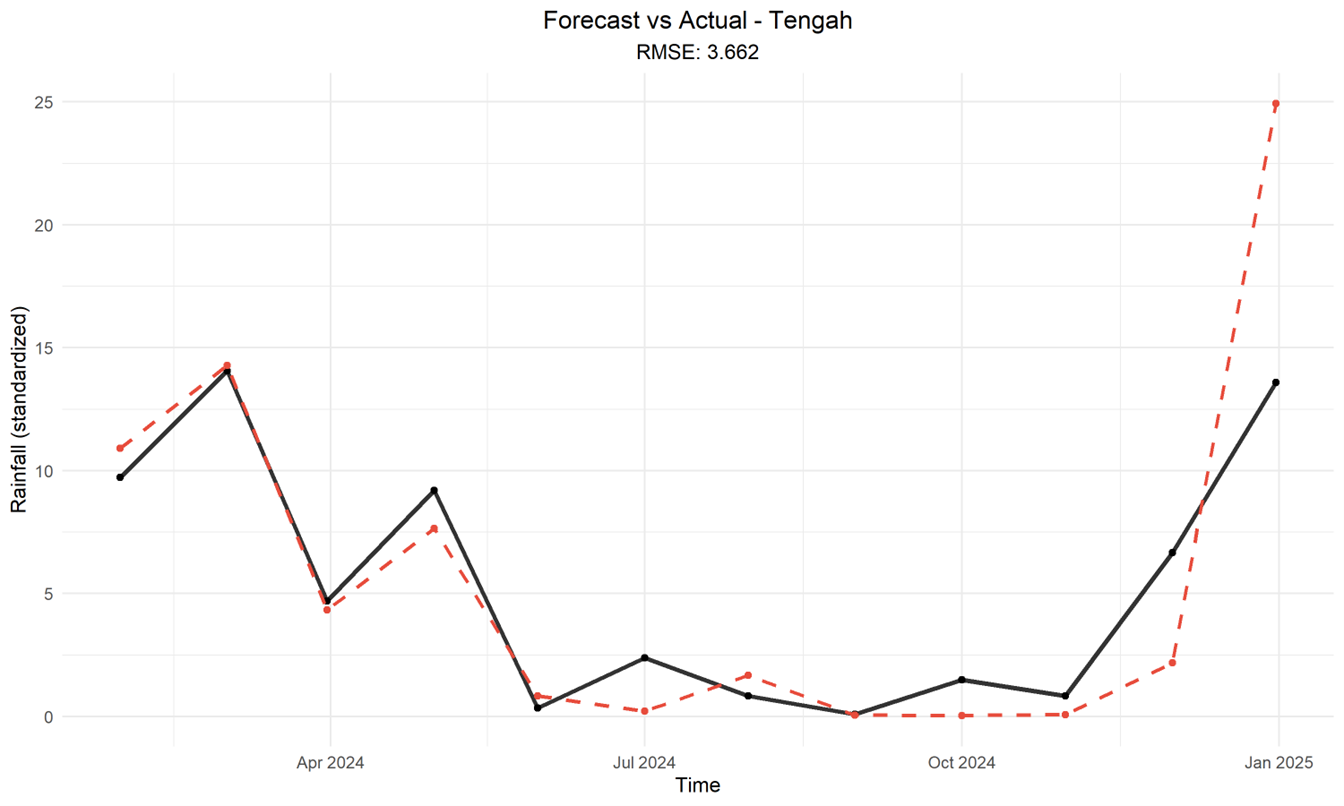
\includegraphics[width=0.9\textwidth]{images/bab_4/bab_4.3/bab_4.3.3/inverse-hasil-forecast-tengah.png}
        \caption{Hasil Peramalan Wilayah Tengah}
        \label{fig:starima-inverse-hasil-forecast-tengah}
    \end{figure}
    Berdasarkan Gambar~\ref{fig:starima-inverse-hasil-forecast-tengah} grafik menunjukkan bahwa model peramalan di Wilayah Tengah mampu merepresentasikan pola temporal dan tren umum curah hujan dengan cukup baik, terutama pada awal hingga pertengahan periode.
    Pada kondisi curah hujan rendah hingga menengah, hasil prediksi relatif mendekati data aktual, menandakan kinerja model yang cukup efektif.
    Namun, pada periode ekstrem di akhir tahun, model cenderung melakukan overestimate terhadap lonjakan curah hujan, sehingga meningkatkan nilai kesalahan prediksi.
    Nilai RMSE sebesar 3,662 menunjukkan bahwa meskipun model berhasil menangkap struktur umum data, akurasinya masih terbatas pada kejadian curah hujan tinggi.
    \begin{figure}[H]
        \centering
        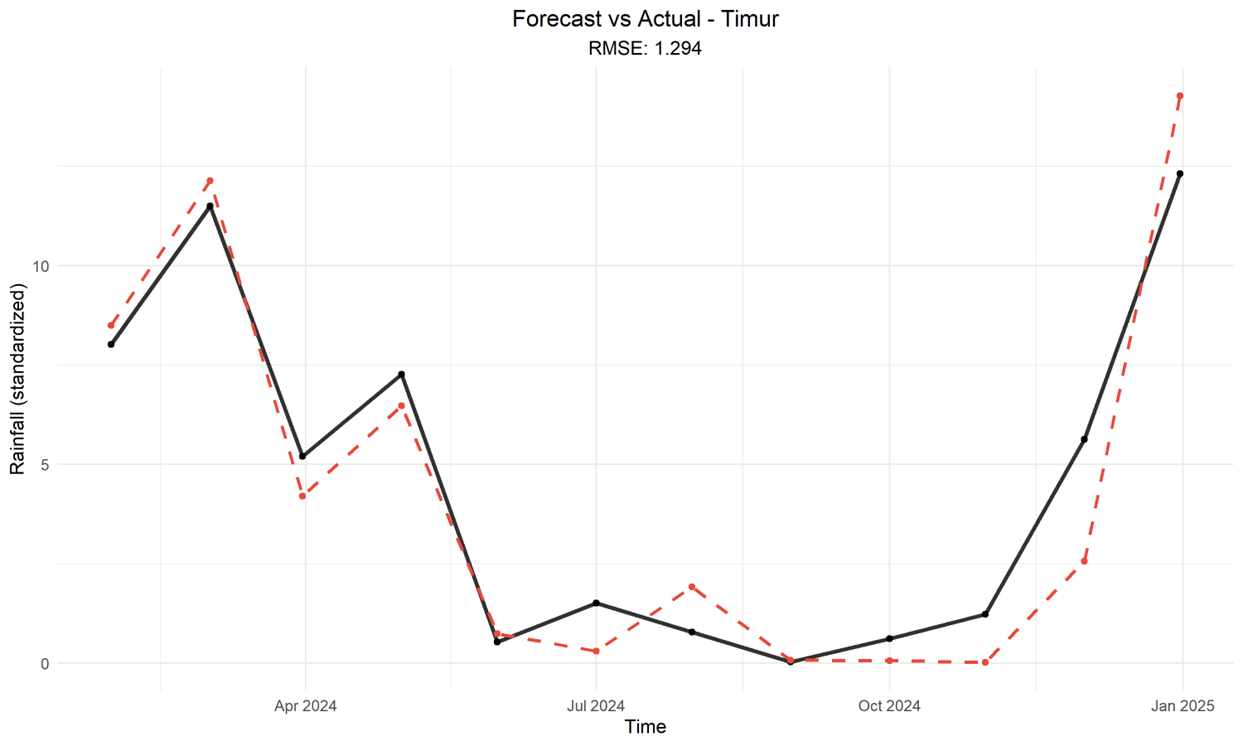
\includegraphics[width=0.9\textwidth]{images/bab_4/bab_4.3/bab_4.3.3/inverse-hasil-forecast-timur.png}
        \caption{Hasil Peramalan Wilayah Timur}
        \label{fig:starima-inverse-hasil-forecast-timur}
    \end{figure}
    Berdasarkan Gambar~\ref{fig:starima-inverse-hasil-forecast-timur} grafik menunjukkan bahwa model peramalan di Wilayah Timur memiliki akurasi sangat tinggi, dengan nilai RMSE sebesar 1,294 yang merupakan paling rendah dibandingkan wilayah lainnya.
    Hasil peramalan sangat mendekati data aktual pada hampir seluruh periode, baik saat curah hujan tinggi maupun rendah.
    Meskipun terdapat sedikit overestimate pada lonjakan di akhir periode, deviasinya relatif kecil dan tidak memengaruhi pola umum.
    Secara keseluruhan, model di Wilayah Timur paling stabil dan representatif, sehingga sangat andal untuk peramalan dan analisis curah hujan.
    \begin{figure}[H]
        \centering
        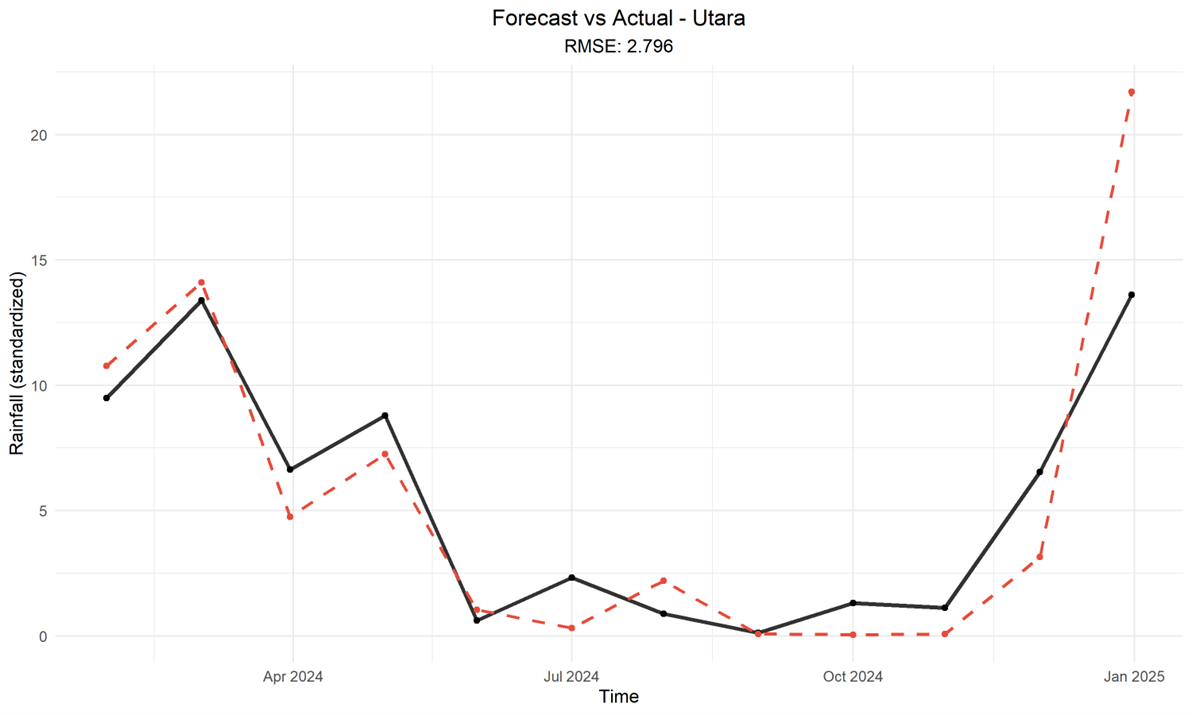
\includegraphics[width=0.9\textwidth]{images/bab_4/bab_4.3/bab_4.3.3/inverse-hasil-forecast-utara.png}
        \caption{Hasil Peramalan Wilayah Utara}
        \label{fig:starima-inverse-hasil-forecast-utara}
    \end{figure}
    Berdasarkan Gambar~\ref{fig:starima-inverse-hasil-forecast-utara} grafik menunjukkan bahwa model peramalan di Wilayah Utara mampu menangkap pola umum curah hujan dengan cukup baik, terutama pada awal hingga pertengahan periode.
    Pada kondisi curah hujan rendah, hasil prediksi relatif mendekati data aktual, menandakan kinerja model yang stabil.
    Namun, pada periode ekstrem di akhir tahun, model cenderung melakukan overestimate terhadap lonjakan curah hujan, sehingga menurunkan akurasi prediksi.
    Nilai RMSE sebesar 2,796 menunjukkan tingkat kesalahan menengah, dengan akurasi yang lebih baik dibandingkan Wilayah Selatan dan Tengah, tetapi masih di bawah Wilayah Timur.
\end{enumerate}
\subsection{Bobot Lokasi Normalisasi Korelasi Silang}
Perhitungan bobot lokasi normalisasi korelasi silang dapat diselesaikan dengan menormalisasikan korelasi silang antar lokasi pada lag yang sesuai, penentuan lag berdasarkan orde struktur data deret waktu.
Perhitungan bobot lokasi normalisasi korelasi silang sesuai dengan Persamaan~\ref{swm_korelasi3}.
Berikut merupakan matriks bobot lokasi normalisasi korelasi silang:
\begin{equation}
    \label{swm-bobot-cross}
    W = 
    \begin{pmatrix}
        0.00 & 0.2504 & 0.2503 & 0.2476 & 0.2518 \\
        0.2508 & 0.00 & 0.2522 & 0.2461 & 0.2509 \\
        0.2507 & 0.2522 & 0.00 & 0.2462 & 0.2509 \\
        0.2509 & 0.2490 & 0.2490 & 0.00 & 0.2510 \\
        0.2517 & 0.2504 & 0.2504 & 0.2476 & 0.00 \\
    \end{pmatrix}
\end{equation}
\begin{enumerate}[label=\Alph*.]
    \item Identifikasi \\
    Setelah mendapatkan bobot, melakukan perhitungan STACF seperti pada Rumus~\ref{st_ma} dan STPACF seperti pada Rumus~\ref{st_ar}.
    Perhitungan Perthitungan STACF dan STPACF ini digunakan untuk menentukan orde $p$, $q$ nya karena data nya sudah di differencing.
    Berikut adalah plot STACF dan STPACF:
    \begin{figure}[H]
        \centering
        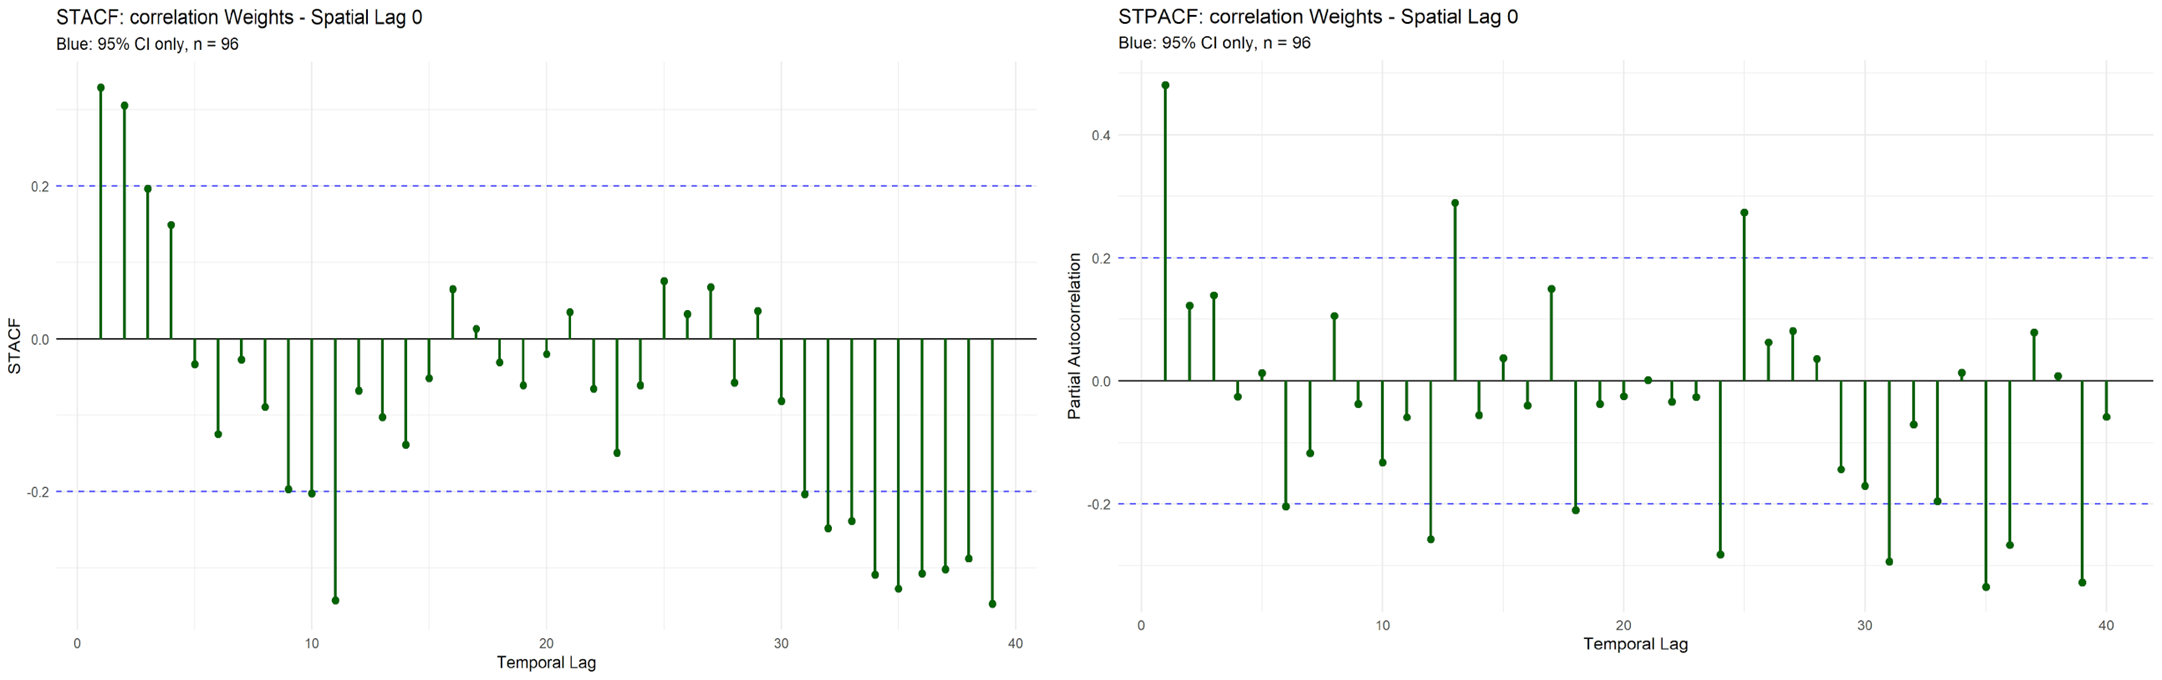
\includegraphics[width=0.9\textwidth]{images/bab_4/bab_4.3/bab_4.3.4/slag-0.png}
        \caption{STACF dan STPACF SLAG 0}
        \label{fig:slag-0-cross}
    \end{figure}
    Gambar~\ref{fig:slag-0-cross} menunjukkan hasil analisis \textit{Spatio-Temporal Autocorrelation Function} (STACF) dan \textit{Spatio Temporal Partial Autocorrelation Function} (STPACF) menggunakan bobot korelasi silang.
    Plot STACF pada spatial lag 0 menunjukkan adanya autokorelasi signifikan pada beberapa lag awal yang meluruh secara bertahap tanpa cut-off yang jelas, mengindikasikan dominasi komponen autoregressive.
    Sementara itu, STPACF memperlihatkan spike signifikan yang kuat pada lag 1 dan tidak signifikan pada lag berikutnya, yang merupakan ciri khas proses AR orde rendah.
    Berdasarkan pola tersebut, model dengan komponen AR(1) tanpa komponen MA yang dominan dinilai paling sesuai untuk merepresentasikan struktur temporal data pada spatial lag 0 dengan pembobotan korelasi silang.
    \begin{figure}[H]
        \centering
        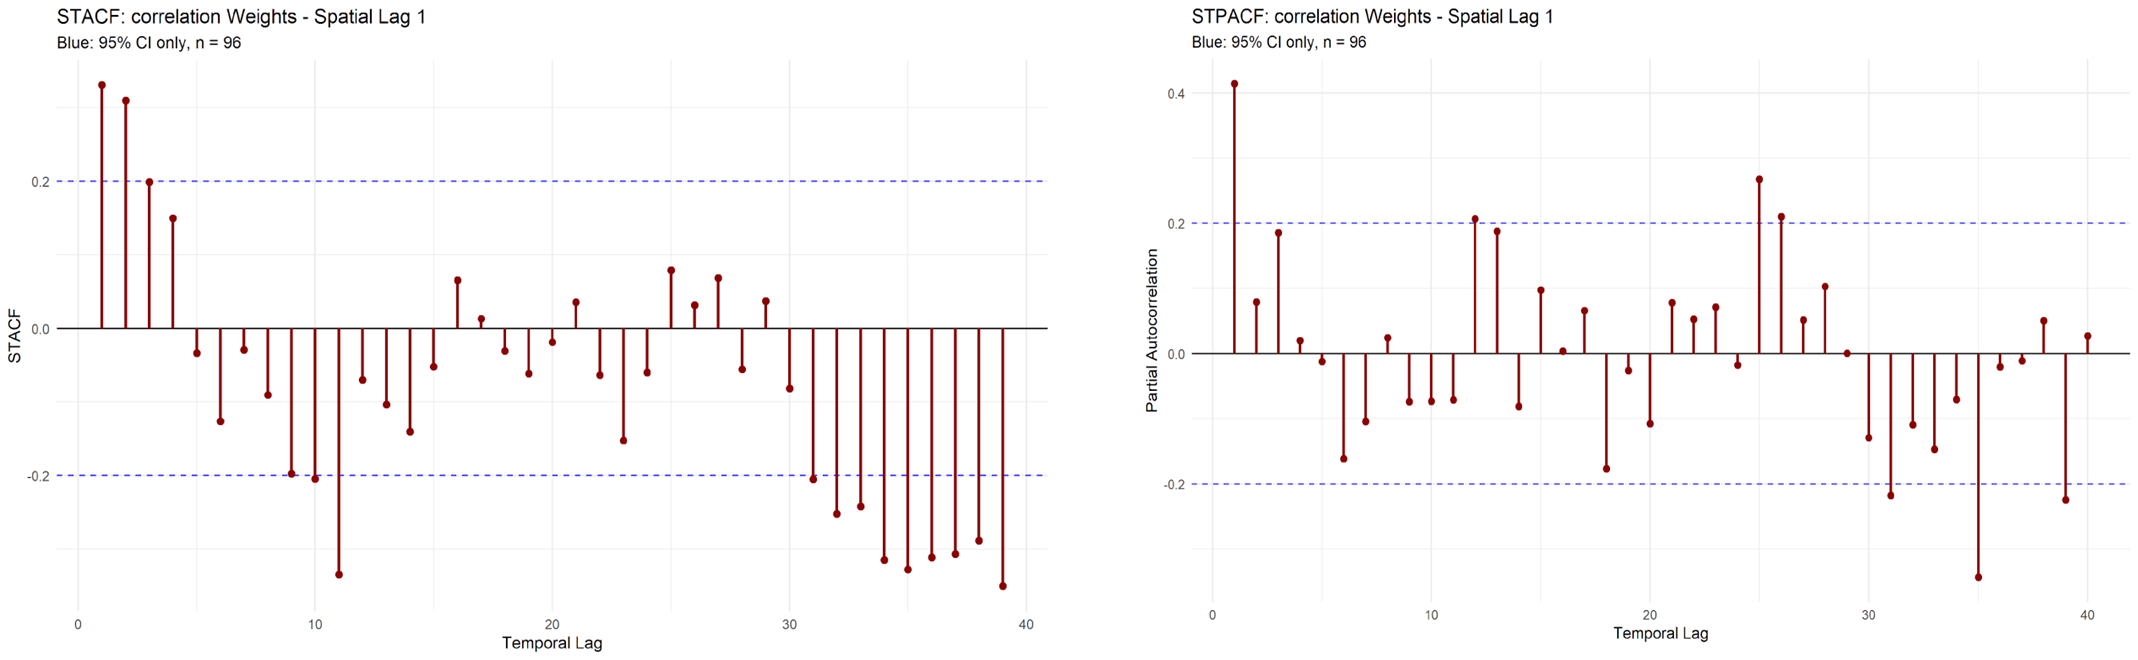
\includegraphics[width=0.9\textwidth]{images/bab_4/bab_4.3/bab_4.3.4/slag-1.png}
        \caption{STACF dan STPACF SLAG 1}
        \label{fig:slag-1-cross}
    \end{figure}
    Gambar~\ref{fig:slag-1-cross} hasil analisis \textit{Spatio Temporal Autocorrelation Function} (STACF) dan \textit{Spatio Temporal Partial Autocorrelation} (STPACF) menggunakan bobot korelasi silang.
    Plot STACF pada spatial lag 1 dengan pembobotan korelasi silang menunjukkan adanya autokorelasi signifikan pada beberapa lag awal yang meluruh secara bertahap, mengindikasikan keberadaan ketergantungan spasio-temporal yang kuat.
    Hal ini menandakan bahwa nilai pengamatan pada suatu wilayah dipengaruhi oleh nilai rata-rata wilayah tetangga pada waktu sebelumnya.
    Sementara itu, STPACF memperlihatkan spike signifikan yang dominan pada lag 1 dan tidak signifikan pada lag berikutnya, yang merupakan ciri proses autoregressive orde satu.
    Berdasarkan pola tersebut, model STARIMA dengan komponen AR spasial orde satu dan tanpa komponen MA yang dominan dinilai paling sesuai untuk merepresentasikan struktur spasio-temporal data.

    \item Estimasi Parameter \\
    Parameter yang diestimasi dari model yang telah diidentifikasi yaitu STARIMA $(0,0,1)(0,1,1)_{12}$ dan STARIMA $(0,0,0)(0,1,1_{0})_{12}$ menggunakan metode Maximum Likelihood, disajikan dalam Tabel~\ref{table:estimasi-paramater-starima-cross}, bersama dengan standar error, nilai $t$, dan nilai $p$ masing-masing:
    \begin{table}[H]
    \centering
    \scriptsize
    \caption{Estimasi Parameter Model STARIMA Bobot Korelasi Silang}
    \label{table:estimasi-paramater-starima-cross}
    \renewcommand{\arraystretch}{1.3}

    \begin{tabular}{|c|c|c|c|c|c|}
        \hline
        \multirow{3}{*}{\textbf{Spatial Order}} &
        \multirow{3}{*}{\textbf{Model}} &
        \multirow{3}{*}{\textbf{Statistik}} &
        \multicolumn{3}{c|}{\textbf{MA Parameter}} \\ \cline{4-6}

        & & &
        \multicolumn{2}{c|}{\textbf{Non Seasonal}} &
        \textbf{Seasonal} \\ \cline{4-6}

        & & &
        \textbf{MA1} & \textbf{MA2} & \textbf{MA} \\
        \hline

        % ================= LAG 0 =================
        \multirow{4}{*}{Lag 0}
        & \multirow{4}{*}{$(0,0,1)\times(0,1,1)_{12}$}
        & Estimasi & 0.374 &  & -0.580 \\ \cline{3-6}
        & & SE      & 0.144 &  & 0.212  \\ \cline{3-6}
        & & t-value & 2.59  &  & -2.73  \\ \cline{3-6}
        & & p-value & 0.0110*** &  & 0.0074*** \\
        \hline

        % ================= LAG 1 =================
        \multirow{4}{*}{Lag 1}
        & \multirow{4}{*}{$(0,0,0)\times(0,1,1_{0})_{12}$}
        & Estimasi &  &  & -0.556 \\ \cline{3-6}
        & & SE      &  &  & 0.22   \\ \cline{3-6}
        & & t-value &  &  & -2.53  \\ \cline{3-6}
        & & p-value &  &  & 0.0131*** \\
        \hline

    \end{tabular}
\end{table}
    Berdasarkan Tabel~\ref{table:estimasi-paramater-starima-cross} hasil estimasi parameter dari kedua model dari lag spasial 0 dan lag spasial 1 yang diestimasi menggunakan metode Maximum Likelihood.
    Masing-masing parameter dilaporkan bersama standar error, nilai $t$, dan nilai $p$ untuk menilai signifikansi statistik.
    Secara umum berdasarkan signifikansi, model STARIMA dengan spatial lag 1 merupakan model terbaik.
    Model ini mampu menangkap ketergantungan spasio-temporal curah hujan antarwilayah melalui komponen MA musiman spasial yang signifikan, dengan struktur yang lebih sederhana dibandingkan model tanpa komponen spasial.
    Oleh karena itu, model spatial lag 1 dipilih sebagai model final untuk proses peramalan.

    \item Model Terbaik \\
    Untuk memilih model spasial terbaik dalam penelitian ini menggunakan evaluasi \textit{Root Mean Squared Error} (RMSE) untuk membandingkan kinerja peramalan dari model-model STARIMA.
    Berdasarkan hasil pada Lampiran~\ref{lampiran:rmse-cross},  berikut adalah tabel nya:
    \begin{table}[H]
    \centering
    \caption{Hasil Model Fitting STARIMA}
    \label{table:hasil-model-fitting-starima-cross}
    \renewcommand{\arraystretch}{1.3}

    \resizebox{\textwidth}{!}{
        \begin{tabular}{lcccc}
            \toprule
            \textbf{Wilayah} &
            \textbf{STARIMA (1,1,0)\textsubscript{0}} &
            \textbf{STARIMA (1,1,1)\textsubscript{0}} &
            \textbf{STARIMA (1,1,0)\textsubscript{1}} &
            \textbf{STARIMA (1,1,1)\textsubscript{1}} \\
            \midrule

            Barat     & 1.689 & 1.652 & 1.685 & 1.653 \\
            Selatan   & 2.019 & 2.003 & 2.018 & 2.005 \\
            Tengah    & 2.066 & 2.125 & 2.066 & 2.120 \\
            Timur     & 1.423 & 1.408 & 1.420 & 1.407 \\
            Utara     & 1.699 & 1.681 & 1.696 & 1.680 \\

            \midrule
            \textbf{Rata-Rata} & 1.7786 & 1.7744 & 1.7776 & 1.7734 \\
            \bottomrule
        \end{tabular}
    }
\end{table}
    Berdasarkan Tabel~\ref{table:hasil-model-fitting-starima-cross} terlihat bahwa evaluasi nilai RMSE per wilayah, model STARIMA $(0,0,0) x (0,1,1_{0})_{12}$ menunjukkan kinerja yang lebih baik pada sebagian besar wilayah secara individual.
    Namun, ditinjau dari nilai RMSE rata-rata, model STARIMA $(0,0,0) x (0,1,1_{0})_{12}$ menghasilkan error yang lebih kecil secara keseluruhan.
    Dengan mempertimbangkan prinsip parsimoni dan kestabilan kinerja global, model STARIMA $(0,0,0) x (0,1,1_{0})_{12}$ dipilih sebagai model terbaik untuk peramalan curah hujan.

    \item Hasil Forecasting \\
    Berikut adalah hasil peramalan menggunakan bobot korelasi silang:
    \begin{figure}[H]
        \centering
        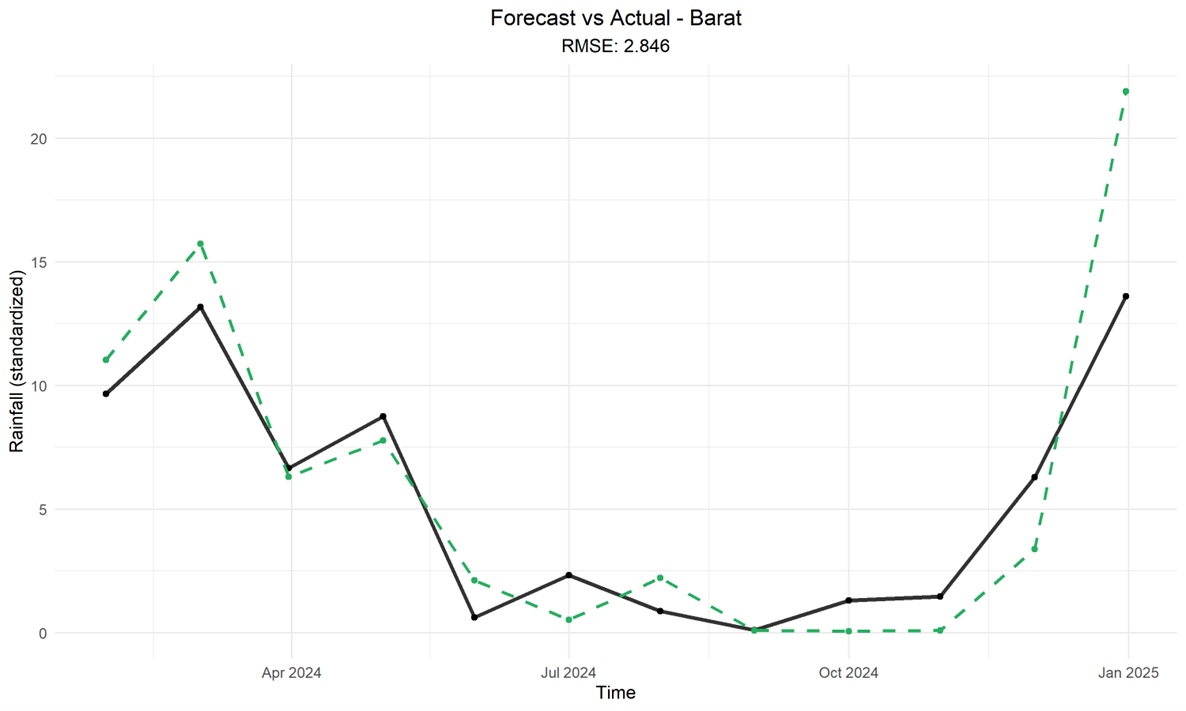
\includegraphics[width=0.9\textwidth]{images/bab_4/bab_4.3/bab_4.3.4/cross-hasil-forecast-barat.png}
        \caption{Hasil Peramalan Wilayah Barat}
        \label{fig:starima-cross-hasil-forecast-barat}
    \end{figure}
    Berdasarkan Gambar~\ref{fig:starima-cross-hasil-forecast-barat} grafik menunjukkan bahwa model peramalan memiliki kinerja cukup baik di Wilayah Barat dengan nilai RMSE sebesar 2,846, yang menandakan kesalahan prediksi relatif kecil.
    Model mampu mengikuti tren utama dan pola musiman curah hujan, terutama pada periode penurunan dari awal hingga pertengahan tahun serta kondisi curah hujan rendah di pertengahan tahun.
    Namun, pada periode dengan perubahan ekstrem, khususnya di awal dan akhir tahun, model cenderung melakukan overestimate, terutama menjelang Januari 2025.
    Secara keseluruhan, model cukup andal dalam menggambarkan pola umum curah hujan, tetapi akurasinya menurun pada lonjakan curah hujan yang tajam, sehingga perlu kehati-hatian dalam interpretasi pada kondisi ekstrem.
    \begin{figure}[H]
        \centering
        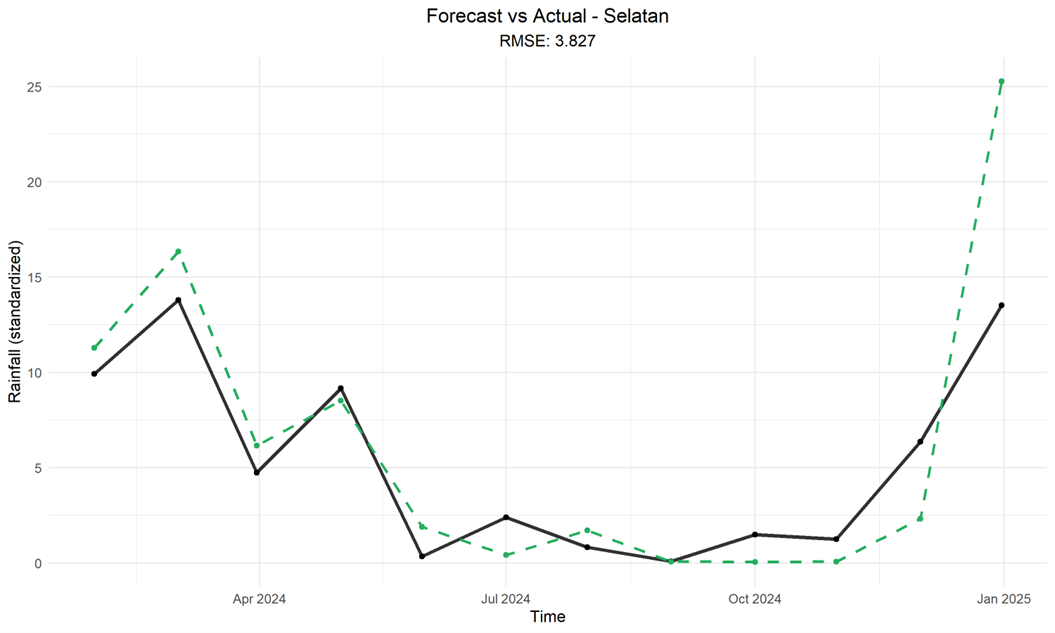
\includegraphics[width=0.9\textwidth]{images/bab_4/bab_4.3/bab_4.3.4/cross-hasil-forecast-selatan.png}
        \caption{Hasil Peramalan Wilayah Selatan}
        \label{fig:starima-cross-hasil-forecast-selatan}
    \end{figure}
    Berdasarkan Gambar~\ref{fig:starima-cross-hasil-forecast-selatan} grafik menunjukkan bahwa kinerja model peramalan di Wilayah Selatan memiliki akurasi yang lebih rendah dibandingkan Wilayah Barat, dengan nilai RMSE sebesar 3,827.
    Model masih mampu mengikuti tren umum dan pola musiman curah hujan, terutama penurunan dari awal hingga pertengahan tahun serta kondisi curah hujan rendah yang relatif stabil.
    Namun, model cenderung kurang presisi dalam menangkap fluktuasi kecil dan melakukan overestimate yang signifikan pada periode ekstrem, khususnya menjelang Januari 2025.
    Deviasi ini menjadi penyumbang utama tingginya nilai RMSE. Secara keseluruhan, model cukup baik untuk analisis pola jangka panjang, tetapi masih memiliki keterbatasan dalam memprediksi lonjakan curah hujan ekstrem di Wilayah Selatan.
    \begin{figure}[H]
        \centering
        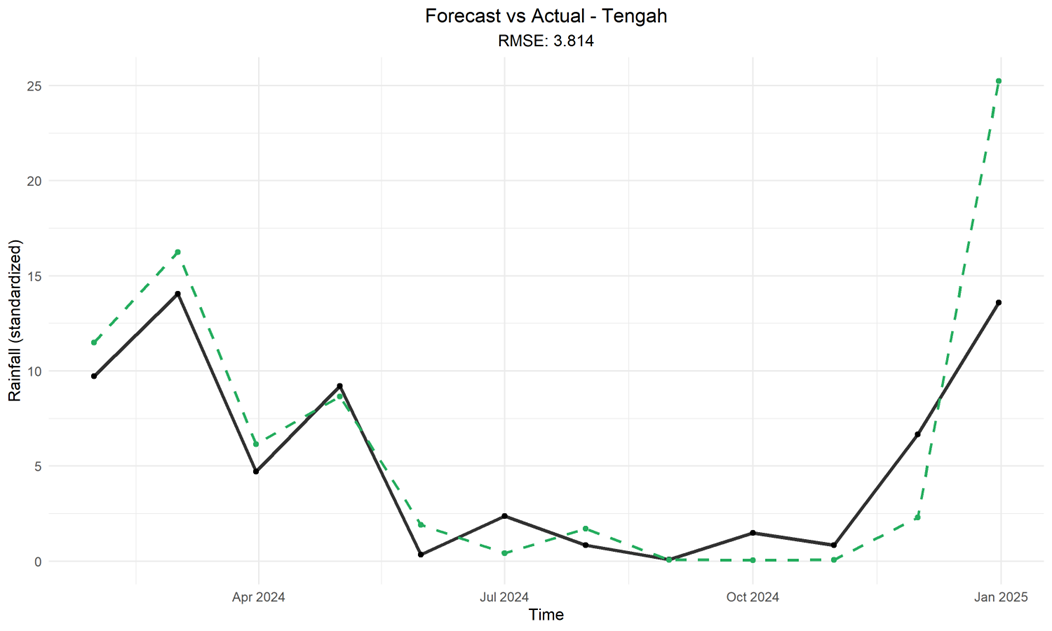
\includegraphics[width=0.9\textwidth]{images/bab_4/bab_4.3/bab_4.3.4/cross-hasil-forecast-tengah.png}
        \caption{Hasil Peramalan Wilayah Tengah}
        \label{fig:starima-cross-hasil-forecast-tengah}
    \end{figure}
    Berdasarkan Gambar~\ref{fig:starima-cross-hasil-forecast-tengah} grafik menunjukkan bahwa model peramalan di Wilayah Tengah memiliki akurasi sedang, dengan nilai RMSE sebesar 3,814 yang sedikit lebih tinggi dibandingkan Wilayah Barat.
    Model mampu mengikuti pola musiman dan tren utama curah hujan, terutama penurunan dari awal hingga pertengahan tahun serta kondisi curah hujan rendah yang stabil pada musim kemarau.
    Namun, model cenderung melakukan overestimate, terutama pada awal dan akhir periode, dengan deviasi paling besar terjadi menjelang Januari 2025 akibat ketidakmampuan model menangkap lonjakan curah hujan ekstrem.
    Secara keseluruhan, model cukup andal untuk analisis pola dan tren jangka panjang, tetapi masih memerlukan pengembangan lebih lanjut untuk meningkatkan akurasi pada peristiwa hujan ekstrem di Wilayah Tengah.
    \begin{figure}[H]
        \centering
        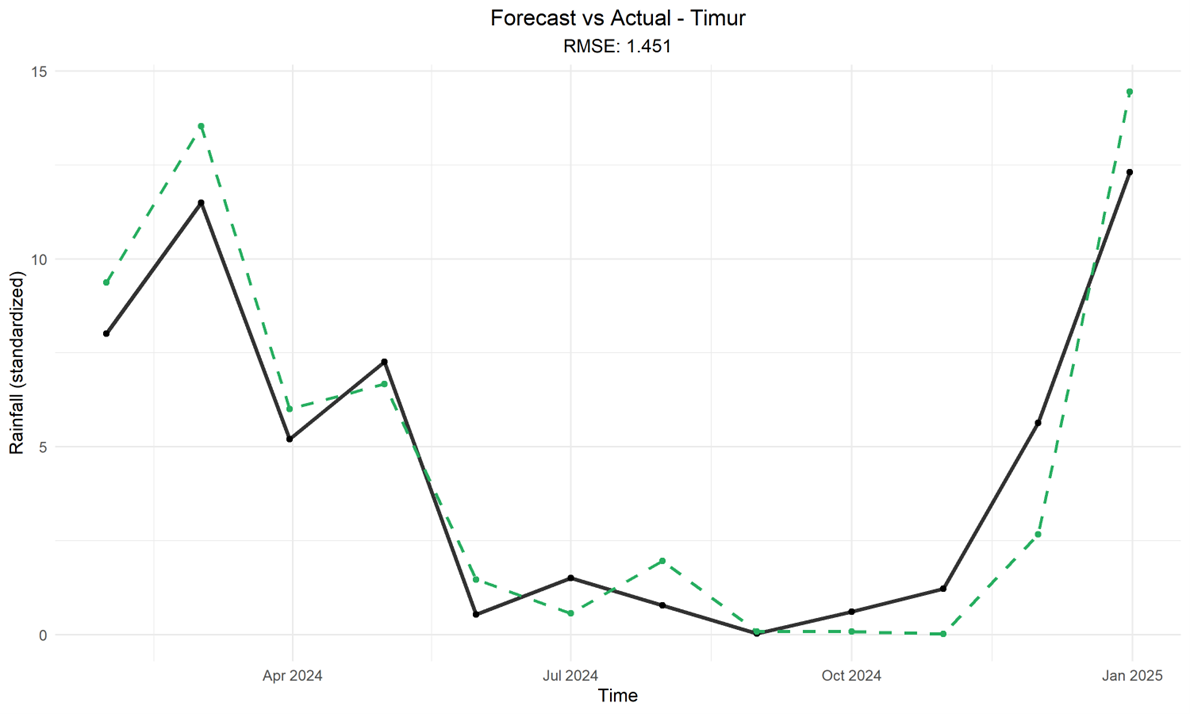
\includegraphics[width=0.9\textwidth]{images/bab_4/bab_4.3/bab_4.3.4/cross-hasil-forecast-timur.png}
        \caption{Hasil Peramalan Wilayah Timur}
        \label{fig:starima-cross-hasil-forecast-timur}
    \end{figure}
    Berdasarkan Gambar~\ref{fig:starima-cross-hasil-forecast-timur} grafik menunjukkan bahwa model peramalan di Wilayah Timur memiliki akurasi sangat baik, dengan nilai RMSE sebesar 1,451 yang merupakan paling rendah dibandingkan wilayah lainnya.
    Model mampu mengikuti pola musiman dan dinamika curah hujan secara konsisten, mulai dari penurunan menuju musim kemarau hingga kenaikan kembali menjelang akhir tahun.
    Perbedaan antara nilai ramalan dan aktual relatif kecil di hampir seluruh periode, dengan hanya sedikit overestimate pada awal dan akhir periode yang tidak signifikan.
    Secara keseluruhan, model di Wilayah Timur paling stabil dan representatif, sehingga sangat layak digunakan untuk peramalan dan analisis curah hujan.
    \begin{figure}[H]
        \centering
        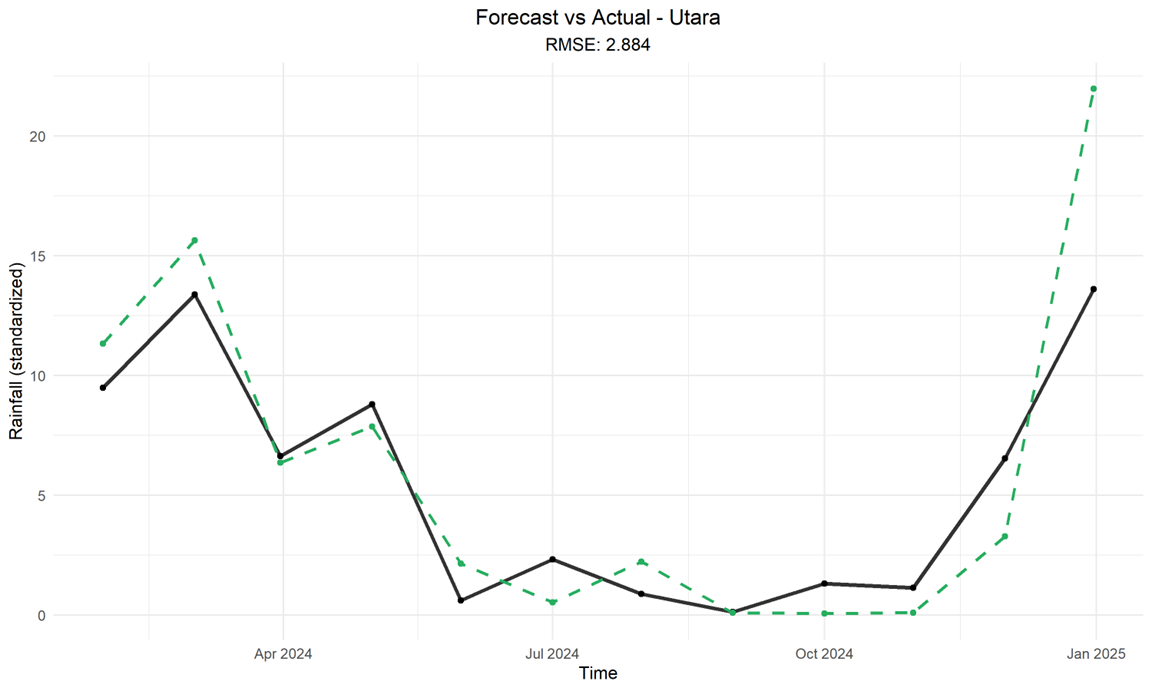
\includegraphics[width=0.9\textwidth]{images/bab_4/bab_4.3/bab_4.3.4/cross-hasil-forecast-utara.png}
        \caption{Hasil Peramalan Wilayah Utara}
        \label{fig:starima-cross-hasil-forecast-utara}
    \end{figure}
    Berdasarkan Gambar~\ref{fig:starima-cross-hasil-forecast-utara} Grafik menunjukkan bahwa model peramalan di Wilayah Utara memiliki akurasi sedang, dengan nilai RMSE sebesar 2,884, lebih baik dibandingkan Wilayah Selatan dan Tengah, namun masih di bawah Wilayah Timur.
    Model mampu mengikuti pola musiman dan tren utama curah hujan, terutama penurunan menuju musim kemarau dan kenaikan kembali di akhir tahun.
    Namun, model cenderung melakukan overestimate, khususnya pada awal dan akhir periode, serta kurang mampu menangkap fluktuasi kecil di pertengahan tahun.
    Secara keseluruhan, model cukup stabil dan layak untuk analisis pola dan peramalan umum, tetapi perlu kehati-hatian dalam memprediksi lonjakan curah hujan ekstrem di Wilayah Utara.
\end{enumerate}